% UPDATES:
% Version 1.2 - JG initial import of text and figures from Google Drive, with edits

\documentclass[11pt]{article}

% packages
%\usepackage{natbib}
%\usepackage{doi}
%\usepackage{hyperref} 
\usepackage[natbibapa]{apacite}
%\usepackage{url}
\usepackage{graphicx}
\usepackage{setspace}
%\usepackage[nolists]{endfloat}
\usepackage{times}
\usepackage{ifthen}
\usepackage{parskip}
\usepackage[font={sf,small},labelfont=bf]{caption}
\usepackage{xspace}
\usepackage[pdftex]{color}
\usepackage{pdfcolmk}
\usepackage{fixltx2e} % for \textsubscript

% line numbers
\usepackage[left]{lineno}

% variable margins
\usepackage[left=2.5cm,top=2.5cm,bottom=3.5cm,right=2.5cm]{geometry}

% this helps figure placement
\renewcommand{\textfraction}{0.0}
\renewcommand{\topfraction}{1}
\renewcommand{\bottomfraction}{1}

% removes filenames from figures
\usepackage{grffile}

% spacing
\setlength{\parindent}{0in} 
\setlength{\parskip}{2\baselineskip}
\linespread{2}
\renewcommand{\baselinestretch}{1.66}\normalsize
%\setstretch{1.5}
%\captionsetup[figure]{font={stretch=1}}

% definitions
\newcommand{\bsf}[1]{\textbf{#1}}
\newcommand{\sem}{S.E.M.\@\xspace}
\newcommand{\degree}{$^o$\@\xspace}
\makeatletter
\setlength{\@fptop}{0pt}
\makeatother

% bib
% \bibliographystyle{apa}
\bibliographystyle{apacite}
\let\cite=\citep
\let\citeN=\citet
\let\citeNP=\citealt
\renewcommand{\bibfont}{\footnotesize}
\setlength{\bibsep}{2pt}

% remove urls from references
\usepackage{etoolbox}
\usepackage{environ}
\newtoggle{bibdoi}
\newtoggle{biburl}
\makeatletter

\undef{\APACrefURL}
\undef{\endAPACrefURL}
\undef{\APACrefDOI}
\undef{\endAPACrefDOI}

\long\def\collect@url#1{\global\def\bib@url{#1}}
\long\def\collect@doi#1{\global\def\bib@doi{#1}}
\newenvironment{APACrefURL}{\global\toggletrue{biburl}\Collect@Body\collect@url}{\unskip\unskip}
\newenvironment{APACrefDOI}{\global\toggletrue{bibdoi}\Collect@Body\collect@doi}{}

\AtBeginEnvironment{thebibliography}{
 \pretocmd{\PrintBackRefs}{%
    {\iftoggle{biburl}{\unskip\unskip doi:\bib@doi}{}}
}{}{}
}

\begin{document}
%change intext citations to ``%'', have to do it after begin document as commands get redefined
\renewcommand{\BBAB}{\BBAA}

{\Large\bf Persistent coding of outcome-predictive cue features in the
  rat nucleus accumbens.}

{\bf Authors}: Jimmie M.\ Gmaz\textsuperscript{1}, James
E.\ Carmichael\textsuperscript{1}, Matthijs A.\ A.\ van der
Meer\textsuperscript{1*}

\textsuperscript{1}Department of Psychological and Brain Sciences,
Dartmouth College, Hanover NH
03755\\ 

\textsuperscript{*}Correspondence should be addressed to MvdM,
Department of Psychological and Brain Sciences, Dartmouth College, 3
Maynard St, Hanover, NH 03755. E-mail: {\sffamily mvdm@dartmouth.edu}.

\textbf{Acknowledgments}: We thank Nancy Gibson, Martin Ryan and Jean
Flanagan for animal care, and Min-Ching Kuo and
Alyssa Carey for technical assistance. This work was supported by
Dartmouth College (Dartmouth Fellowship to JMG and JEC, and start-up funds to
MvdM) and the Natural Sciences and Engineering Research Council
(NSERC) of Canada (Discovery Grant award to MvdM, Canada Graduate
Scholarship to JMG).

\textbf{Conflict of Interest}: The authors declare no competing
financial interests.\\

\newpage
\linenumbers

\section*{Abstract}

The nucleus accumbens (NAc) has been shown to be important for
learning from feedback, and biasing and invigorating behavior in
response to outcome-predictive cues. NAc encodes outcome-related cue
features such as the magnitude and identity of reward. However, not
much is known about how features of cues themselves are encoded.  We
designed a decision making task where rats learned multiple sets of
outcome-predictive cues, and recorded single-unit activity in the NAc
during performance. We found that coding of various cue features
occurred alongside coding of expected outcome. Furthermore, this
coding persisted both during a delay period, after the rat made a decision
and was waiting for an outcome, and after the outcome was
revealed. Encoding of cue features in the NAc may enable contextual
modulation of ongoing behavior, and provide an eligibility trace of
outcome-predictive stimuli for updating stimulus-outcome associations
to inform future behavior.

\newpage

\section*{Introduction}

Theories of nucleus accumbens (NAc) function generally agree that this
brain structure contributes to motivated behavior, with some
emphasizing a role in learning from reward prediction errors (RPEs) (\citeNP{Joel2002,Maia2009,Khamassi2012,Lee2012,Schultz2016,Averbeck2017}; see
  also the addiction literature on effects of drug
  rewards; \citeNP{Kalivas2005,Hyman2006,Carelli2009}) and others a role in
the modulation of ongoing behavior through stimuli associated with
motivationally relevant outcomes \cite[invigorating,
  directing;][]{Nicola2010a,Salamone2012,Floresco2015}. These
proposals echo similar ideas on the functions of the neuromodulator
dopamine \cite{Maia2009,Berridge2012,Salamone2012,Schultz2016}, with
which the NAc is tightly linked functionally as well as anatomically
\cite{Cheer2007,Ikemoto2007,DuHoffmann2014,Takahashi2016}.

Much of our understanding of NAc function comes from studies of how
cues that predict motivationally relevant outcomes (e.g.\ reward)
influence behavior and neural activity in the NAc. Task designs that
associate such cues with rewarding outcomes provide a convenient
access point eliciting conditioned responses such as sign-tracking and
goal-tracking \cite{hearst1974sign,Robinson2009},
pavlovian-instrumental transfer \cite{Estes1943,Rescorla1967} and
enhanced response vigor \cite{Niv2007,Nicola2010a}, which tend to be
affected by NAc manipulations (\citeNP{Corbit2011,Flagel2011,Chang2012};
although not always
  straightforwardly; \citeNP{Giertler2004,Chang2013}). Similarly, analysis
of RPEs typically proceeds by establishing an association between a
cue and subsequent reward, with NAc responses transferring from
outcome to the cue with learning
\cite{Schultz1997,Setlow2003,Roitman2005,Day2007a}.

Surprisingly, although substantial work has been done on the coding of
outcomes predicted by such cues
\cite{Hollerman1998,Setlow2003,Nicola2004,Roitman2005,Day2006,Roesch2009a,Saddoris2011,Goldstein2012,Lansink2012,Bissonette2013,McGinty2013,Atallah2014,Sugam2014,Cooch2015,West2016},
much less is known about how outcome-predictive cues themselves are
encoded in the NAc \cite[but see;][]{Sleezer2016}. This is an important issue for
at least two reasons. First, in reinforcement learning, motivationally
relevant outcomes are typically temporally delayed relative to the
cues that predict them. In order to solve the problem of assigning
credit (or blame) across such temporal gaps, some trace of preceding
activity needs to be maintained \cite{sutton1998,Lee2012}. For
example, if you become ill after eating food X in restaurant A,
depending on if you remember the identity of the restaurant or the
food at the time of illness, you may learn to avoid all restaurants,
restaurant A only, food X only, or the specific pairing of
X-in-A. Therefore, a complete understanding of what is learned
following feedback requires understanding what “trace” is
maintained. Since NAc is a primary target of DA signals interpretable
as RPEs, and NAc lesions impair RPEs
related to timing, its activity trace will help determine what can be
learned when RPEs arrive
\cite{Ikemoto2007,McDannald2011,Hart2014,Hamid2016,Takahashi2016}.


Second, for ongoing behavior, the relevance of cues typically depends
on “context”. In experimental settings, context may include the
identity of a preceding cue, spatial or configural arrangements
\cite{Holland1992,Bouton1993,Honey2014}, and unsignaled rules as
occurs in set shifting and other cognitive control tasks
\cite{Grant1948,cohen1992context,Floresco2006a,Sleezer2016}. In such
situations, the question arises how selective, context-dependent
processing of outcome-predictive cues is implemented. For instance, is
there a “gate” prior to NAc such that only currently relevant cues are encoded in NAc, or are all cues represented in NAc but
their current values dynamically updated
\cite{Goto2008,Fitzgerald2014,Sleezer2016}. Representation of cue
identity would allow for context-dependent mapping of outcomes
predicted by specific cues.

Thus, both from a learning and a flexible performance perspective, it
is of interest to determine how cue identity is represented in the
brain, with NAc of particular interest given its anatomical and
functional position at the center of motivational systems. We sought
to determine whether cue identity is represented in the NAc, if cue
identity is represented alongside other motivationally relevant
variables, such as cue value, and if these representations are
maintained after a behavioral decision has been made (Figure
\ref{fig:schematic}). To address these questions, we recorded the
activity of NAc units as rats performed a task in which multiple,
distinct sets of cues predicted the same outcome.


 \begin{figure}[ht!]
\centering
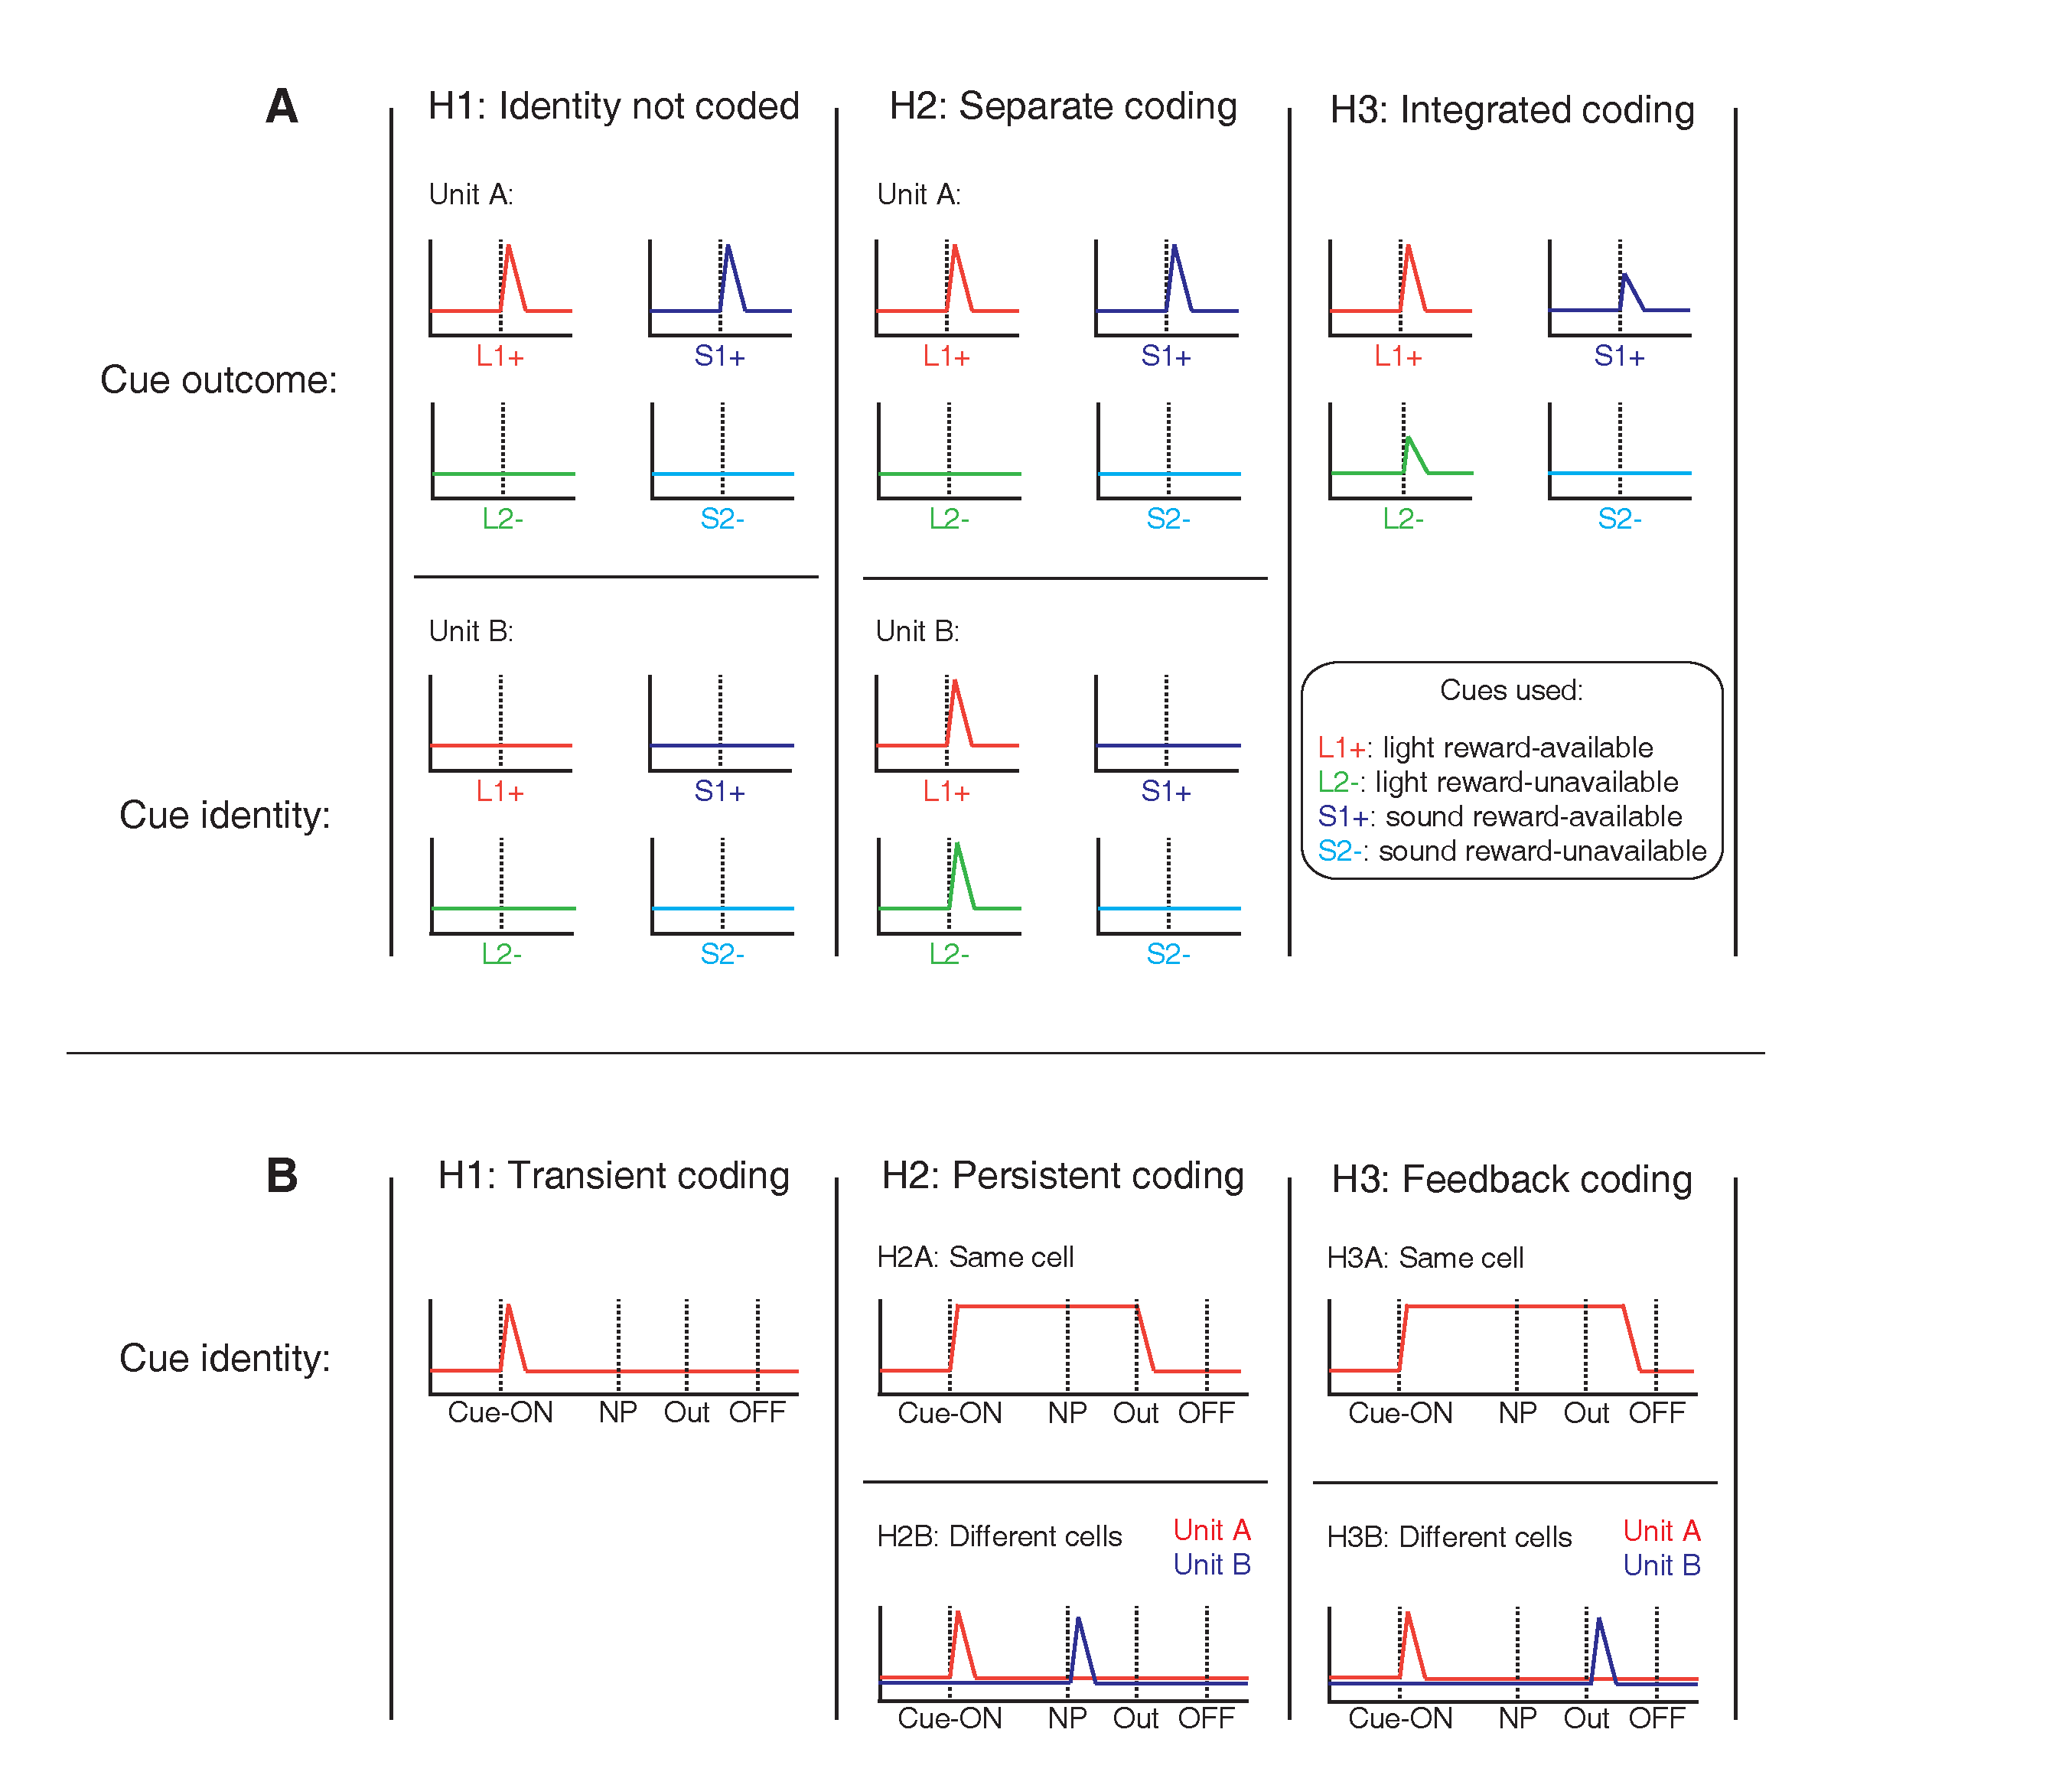
\includegraphics[width=\textwidth]{Fig 1 - Schematic neural.pdf}
\caption{
Schematic of potential coding strategies for cue identity
  (light, sound) and cue outcome (reward-available,
  reward-unavailable) employed by single units in the NAc across
  different units (A) and in time (B). \bsf{A}: Displayed are
  schematic PETHs illustrating putative responses to different cues
  under different hypotheses of how cue identity and outcome are
  coded. H1 (left panel): Coding of cue identity is absent in the
  NAc. Top: Unit A encodes a motivationally relevant variable, such as
  expected outcome, similarly across other cue features, such as cue
  identity or physical location. Hypothetical plot is firing rate
  across time. L1+ (red) signifies a reward-available light cue, S1+
  (navy blue) a reward-available sound cue, L2- (green) a
  reward-unavailable light cue, S2- (light blue) a reward-unavailable
  sound cue. Dashed line indicates onset of cue. Bottom: No units
  within the NAc discriminate their firing according to cue
  identity. H2 (middle panel): Coding of cue identity occurs
  independently of encoding of motivationally relevant variables such
  as expected outcome or subsequent vigor. Top: Same as H1, with unit
  A discriminating between reward-available and reward-unavailable
  cues. Bottom: Unit B discriminates firing across stimulus
  modalities, depicted here as firing to light cues but not sound
  cues. H3 (right panel): Coding of cue identity is integrated with
  coding of other motivationally relevant variables. Hypothetical
  example demonstrating a unit that responds to outcome-predictive
  cues, but firing rate is also modulated by cue identity, firing most
  for the reward-available light cue. \bsf{B}: Displayed are schematic
  PETHs illustrating potential ways in which cue identity signals may
  persist over time. H1 (left panel): Cue-onset triggers a transient
  response to a unit that codes for cue identity. Dashed lines
  indicate time of a behavioral or environmental event. 'Cue-ON'
  signifies onset of cue, 'NP' signifies when the rat holds a nosepoke
  at a reward receptacle, 'Out' signifies when the outcome is
  revealed, 'OFF' signifies when the cue turns off. H2 (middle
  panel): Coding of cue identity persists during a nosepoke hold
  period until outcome is revealed. Coding can either be maintained by
  the same unit as during cue-onset (H2A) or by a sequence of units
  (H2B). H3 (right panel): Coding of cue identity persists after the outcome is received when the rat gets feedback about his decision,
  by either the same unit as during cue-onset (H3A) or by a sequence of units (H3B). The
  same hypotheses apply to other information-containing aspects of the
  environment when the cue is presented, such as the physical location
  of the cue.}
\label{fig:schematic}
\end{figure} \clearpage

\section*{Results}

\subsection*{Behavior}

Rats were trained to discriminate between cues signaling the
availability and absence of reward on a square track with four
identical arms for two distinct set of cues (Figure
\ref{fig:task}). During each session, rats were presented sequentially
with two behavioral blocks containing cues from different sensory
modalities, a light and a sound block, with each block containing a
cue that signalled the availability of reward (reward-available), and
a cue that signalled the absence of reward (reward-unavailable). To
maximize reward receipt, rats should approach reward sites on
reward-available trials, and skip reward sites on reward-unavailable
trials (see Figure \ref{fig:behav}A for an example learning
curve). All four rats learned to discriminate between the
reward-available and reward-unavailable cues for both the light and
sound blocks as determined by reaching significance ($p <$ .05) on a
daily chi-square test comparing approach behavior for reward-available
and reward-unavailable cues for each block, for at least three
consecutive days (range for time to criterion: 22 - 57
days). Maintenance of behavioral performance during recording sessions
was assessed using linear mixed effects models for both proportion of
trials where the rat approached the receptacle, and trial
length. Analyses revealed that the likelihood of a rat to make an
approach was influenced by whether a reward-available or reward-unavailable cue was presented, but was not significantly modulated by whether the rat was presented with a light or sound cue (Percentage
approached: light reward-available = 97\%; light reward-unavailable =
34\%; sound reward-available = 91\%; sound reward-unavailable 35\%; cue identity p
$=$ .115; cue outcome p$<$ .001; Figure \ref{fig:behav}B). A similar trend was seen with the
length of time taken to complete a trial (Trial length: light
reward-available = 1.85 s; light reward-unavailable = 1.74 s; sound
reward-available = 1.91 s; sound reward-unavailable 1.78 s; cue identity p $=$ .106; cue outcome p $<$ .001; Figure \ref{fig:behav}C). Thus, during recording, rats successfully
discriminated the cues according to whether or not they signaled the
availability of reward at the reward receptacle.

 \begin{figure}[ht!]
\centering
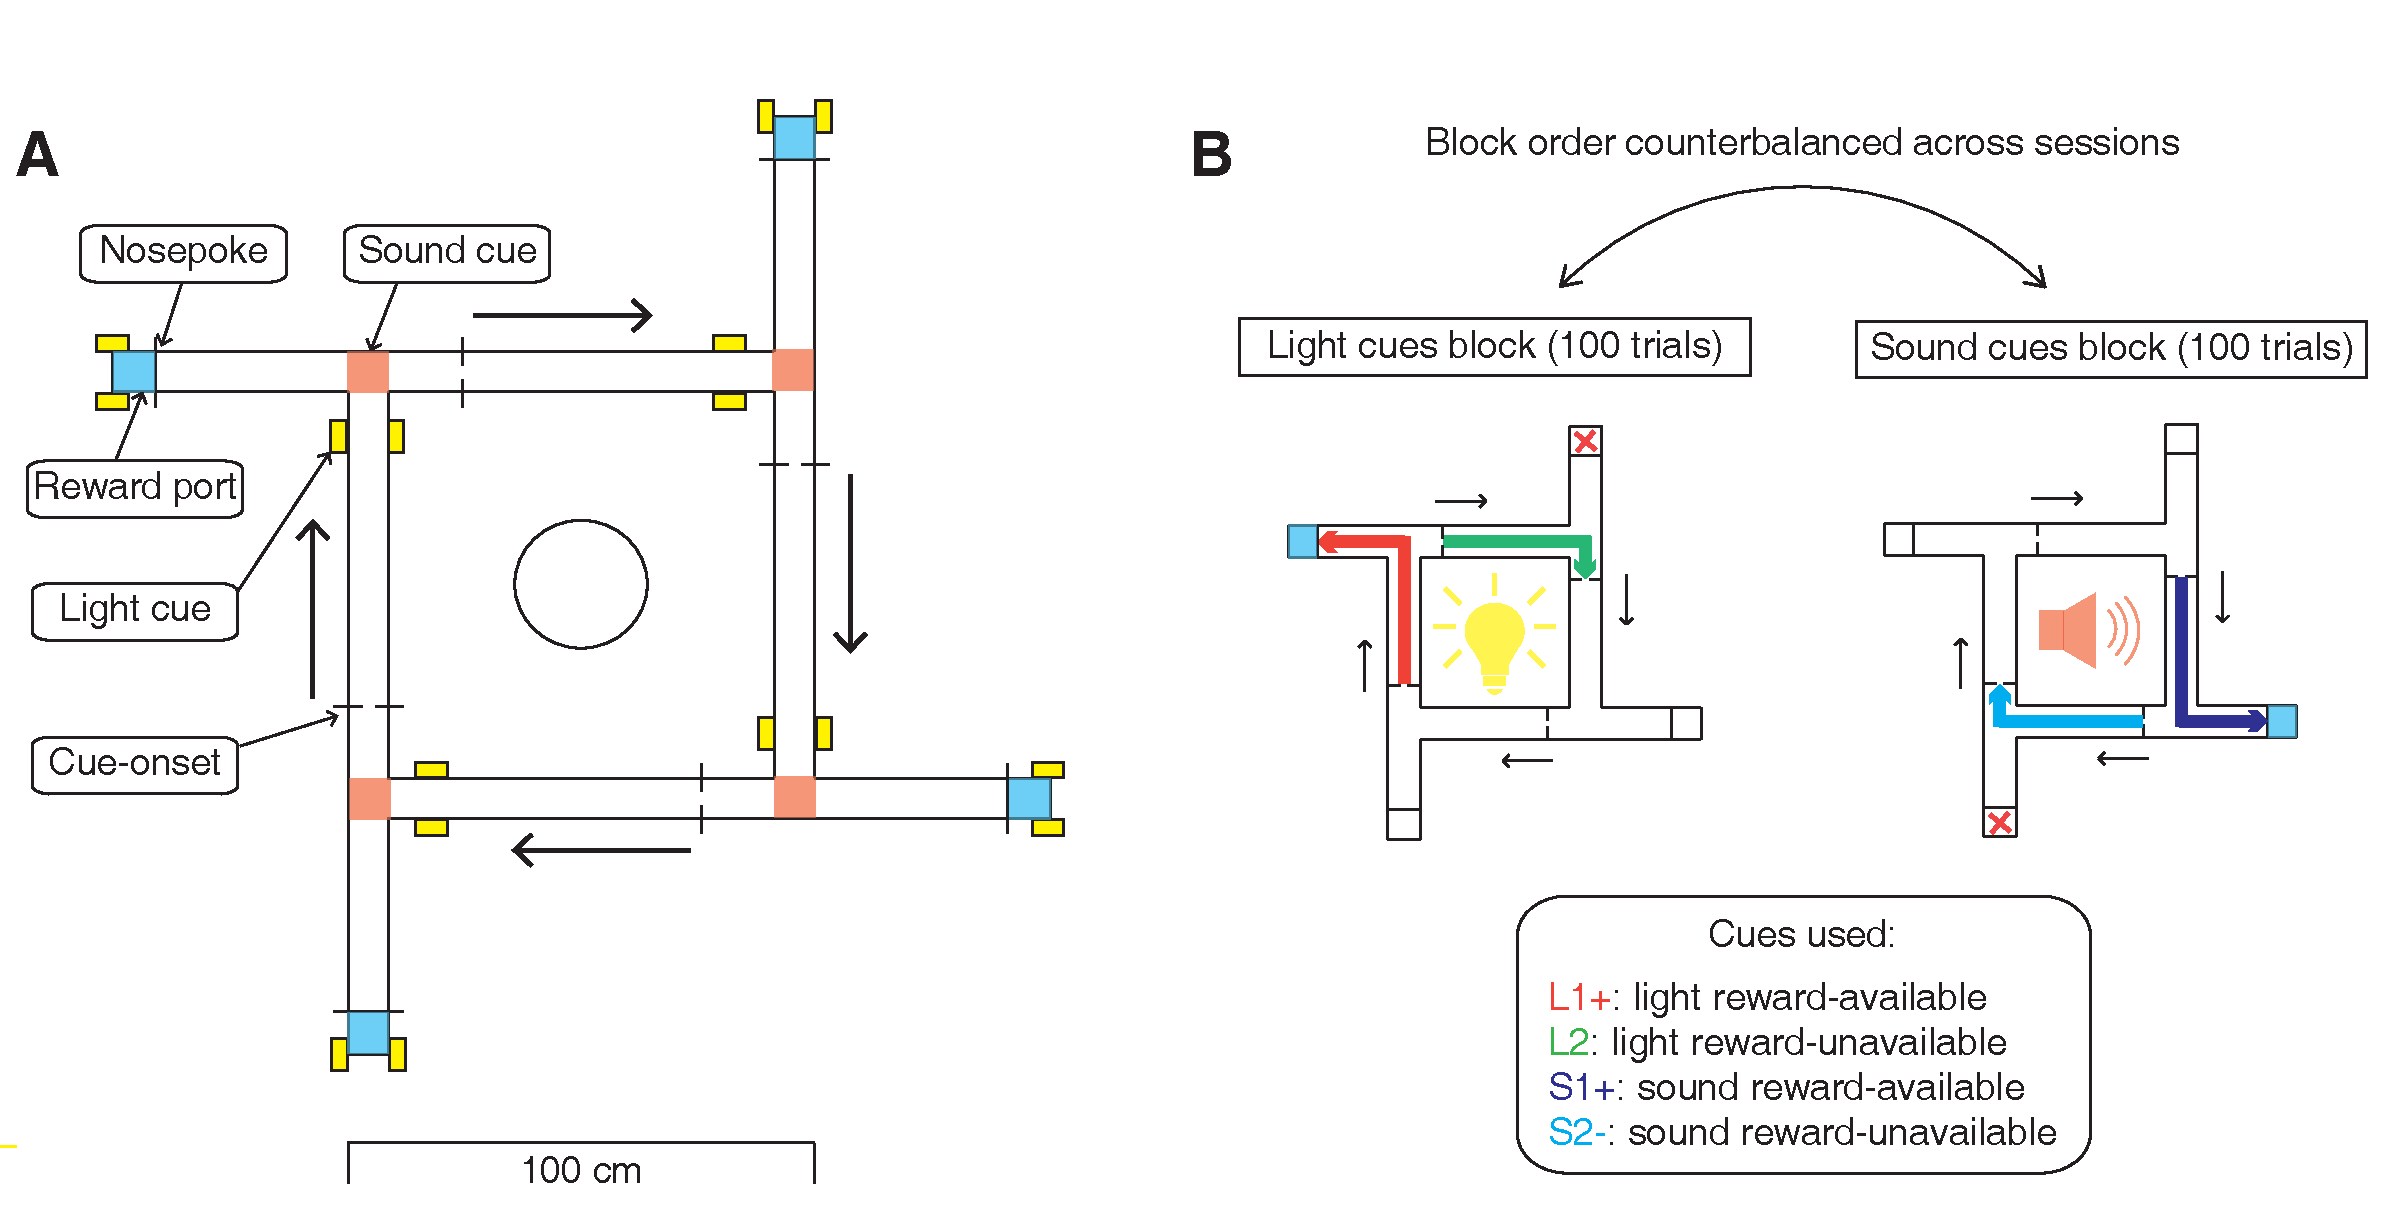
\includegraphics[width=\textwidth]{Fig 2 - Schematic task.pdf}
\caption{Schematic of behavioral task. \bsf{A}: To scale depiction of square
track consisting of multiple identical T-choice points. At each choice point,
the availability of 12\% sucrose reward at the nearest reward receptacle (light
blue fill) was signaled by one of four possible cues, presented when the rat
initiated a trial by crossing a photobeam on the track (dashed
lines). Photobeams at the ends of the arms by the receptacles registered
Nosepokes (solid lines). Rectangular boxes with yellow fill indicate location of LEDs used
for light cues. Speakers for tone cues were placed underneath the choice
points, indicated by magenta fill on track. Arrows outside of track indicate correct running direction. Circle in the center indicates location of pedestal during pre- and post-records. Scale bar is located beneath the track. \bsf{B}: Progression of
a recording session. A session was started with a 5 minute recording period on
a pedestal placed in the center of the apparatus. Rats then performed the light and sound blocks of the cue discrimination task in succession for 100 trials each, followed by another 5 minute recording period on the pedestal. Left in figure depicts a light block, showing an
example trajectory for a correct reward-available (approach trial; red) and reward-unavailable
(skip trial; green) trial. Right in figure depicts a sound block, with a reward-available
(approach trial; navy blue) and reward-unavailable (skip trial; light blue) trial. Ordering of the light and sound blocks was counterbalanced across sessions. Reward-available and reward-unavailable cues were presented pseudo-randomly, such that not more than two of the same type of cue could be presented in a row. Location of the cue on the track was irrelevant for
behavior, all cue locations contained an equal amount of reward-available and
reward-unavailable trials.
}
\label{fig:task}
\end{figure} \clearpage

 \begin{figure}[ht!]
\centering
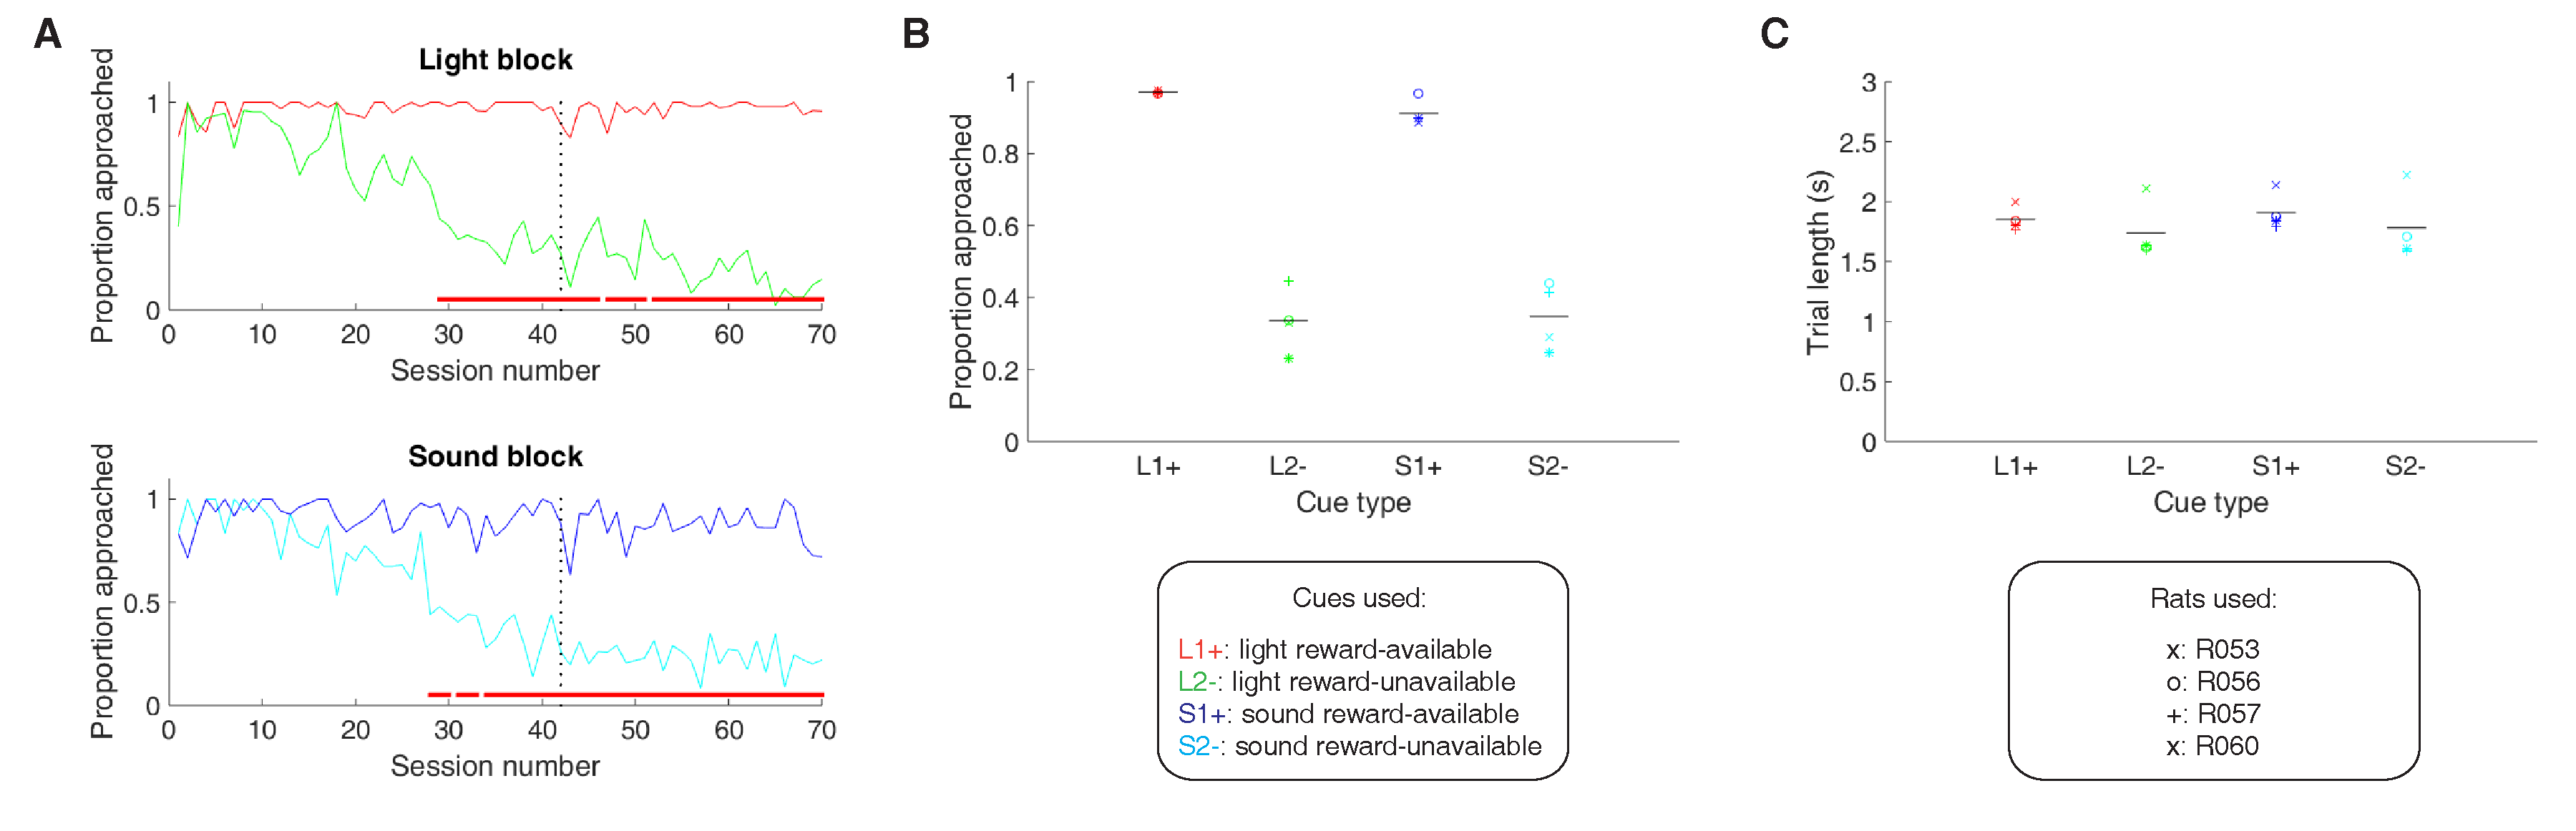
\includegraphics[width=\textwidth]{Fig 4 - Behavioral results.pdf}
\caption{Performance on the behavioral task. \bsf{A}. Example learning curves
across sessions from a single subject (R060) showing the proportion approached
for reward-available (red line for light block, navy blue line for sound
block) and reward-unavailable trials (green line for light block, light blue
line for sound block) for light (top) and sound (bottom) blocks. Fully correct performance corresponds to an approach
proportion of 1 for reward-available trials and 0 for reward-unavailable
trials. Rats initially approach on both reward-available and
reward-unavailable trials, and learn with experience to skip non-rewarded
trials. Red bars indicate days in which a rat statistically discriminated
between reward-available and reward-unavailable cues, determined by a chi
square test. Dashed line indicates time of electrode implant
surgery. \bsf{B-C}: Summary of performance during recording sessions for each
rat. \bsf{B}: Proportion approached for all rats, averaged across all
recording sessions. Different columns indicate the different cues
(reward-available (red) and reward-unavailable (green) light cues,
reward-available (navy blue) and reward-unavailable (light blue) sound
cues). Different symbols correspond to individual subjects; horizontal black
line shows the mean. All rats learned to discriminate between reward-available
and reward-unavailable cues, as indicated by the clear difference of
proportion approached between reward-available ($\sim$90\% approached) and
reward-unavailable cues ($\sim$30\% approached), for both blocks (see Results
for statistics). \bsf{C}: Average trial length for each cue. Note that the
time to complete a trial was comparable for the different cues.}
\label{fig:behav}
\end{figure} \clearpage

\subsection*{NAc units encode behaviorally relevant and irrelevant cue features}

{\bf Single unit responses discriminate cue features:}

We sought to address which parameters of our task were encoded by NAc activity,
specifically whether the NAc encodes aspects of motivationally relevant cues not
directly tied to reward, such as the identity and location of the cue, and
whether this coding is independent or integrated with coding of cue outcome. To
do this we recorded a total of 443 units with $>$ 200 spikes in the NAc from 4
rats over 57 sessions (range: 12 - 18 sessions per rat) while they performed a cue discrimination task (Table
\ref{tbl1}). Units that exhibited a drift in firing rate over the course of
either block were excluded from further analysis, leaving 344 units for further
analysis. The activity of 133 (39\%) of these 344 units were modulated by the
cue, with more showing a decrease in firing (n = 103) than an increase (n = 30)
around the time of cue-onset (Table \ref{tbl1}). Within this group, 24 were
classified as FSIs, while 109 were classified as SPNs. Upon visual inspection,
we observed several patterns of firing activity, including units that
discriminated firing upon cue-onset across various cue conditions, showed
sustained differences in firing across cue conditions, had transient responses
to the cue, showed a ramping of activity starting at cue-onset, and showed
elevated activity immediately preceding cue-onset, for example (Figure
\ref{fig:examples}). To characterize more formally whether these cue-evoked
responses were modulated by various aspects of the task, we fit a GLM to each
cue-modulated unit. Fitting GLMs revealed that a variety of task parameters
accounted for a significant portion of firing rate variance in NAc cue-modulated
units (Figure \ref{fig:GLM}, Table \ref{tbl1}). Notably, there were units that
discriminated between whether the rat was performing in the light or sound block
(28\% of cue-modulated units, accounting for 6\% of variance on average), which
arm the rat was currently on (38\% of cue-modulated units, accounting for 6\% of
variance on average), and whether the rat was engaged in the common portion of a
reward-available or reward-unavailable trial (26\% of cue-modulated units,
accounting for 4\% of variance on average), suggesting that the NAc
encodes features of reward-predictive cues separate from expected
outcome (Figure \ref{fig:examples}A-F). Furthermore, overlap of coding of cue
features within units was not different than expected by chance according to
chi-square tests, suggesting for integrated coding across various aspects of a
cue (Figure \ref{fig:examples}G,H). Additionally, a sliding window GLM centered on cue-onset revealed that cue identity and cue location contributed to the activity
of a significant proportion of cue-modulated units throughout this epoch, whereas an increase in units encoding cue outcome became apparent after cue-onset (Figure \ref{fig:GLM}D).  Together, these findings show that various cue features are represented in the NAc, 
and that this coding is both integrated and separate from expected outcome (Figure
\ref{fig:schematic}; H2,H3).

\begin{table}[p]
\centering
\setlength{\tabcolsep}{1 em} % for the horizontal padding
\begin{tabular}{l c  c c c c}

\bsf{Task parameter}                                 & \bsf{Total}        & \bsf{$\uparrow$ MSN}        & \bsf{$\downarrow$ MSN}        & \bsf{$\uparrow$ FSI}       & \bsf{$\downarrow$ FSI}\\
\hline
All units                       & 443        & 155         & 216          & 27          & 45\\
\hline
\textit{Rat ID}                       &         &       &          &          &\\
\hline
\hspace{3mm}R053                       & 145         & 51          & 79          & 4         & 11\\
\hline
\hspace{3mm}R056                       & 70         & 12          & 13         & 17          & 28\\
\hline
\hspace{3mm}R057   	          & 136         & 55          & 75          & 3          & 3\\
\hline
\hspace{3mm}R060                       & 92         & 37          & 49          & 3          & 3\\
\hline 
Analyzed units                       & 344        & 117         & 175         & 18         & 34\\
\hline
Cue modulated units                      & 133         &24          &85          & 6          &18\\
\hline
\hspace{3mm}\textit{GLM aligned to cue-onset}                       &         &       &          &          &\\
\hline
\hspace{6mm}Cue identity       & 37         & 7          & 21          & 1          & 8\\
\hline
\hspace{6mm}Cue location       & 50         &13          & 27          & 3          & 7\\
\hline
\hspace{6mm}Cue outcome       & 34         & 10          & 18        & 0          & 6\\
\hline
\hspace{6mm}Approach behavior      & 31         & 8          & 18          & 1          & 4\\
\hline
\hspace{6mm}Trial length       & 25        & 5          & 18         & 0         & 2\\
\hline
\hspace{6mm}Trial number       & 32         & 11          & 12         & 1          & 8\\
\hline
\hspace{6mm}Previous trial       & 5         & 0          &5          & 0          & 0\\
\hline
\hspace{3mm}\textit{GLM aligned to nosepoke}                       &         &       &          &          &\\
\hline
\hspace{6mm}Cue identity       & 66         &14          & 36          & 2          &14\\
\hline
\hspace{6mm}Cue location       & 66         &14          & 40          & 3          & 9\\
\hline
\hspace{6mm}Cue outcome       & 42        & 8          & 29        & 0          & 5\\
\hline
\hspace{3mm}\textit{GLM aligned to outcome}                       &         &       &          &          &\\
\hline
\hspace{6mm}Cue outcome       & 10        & 0          & 6       & 0          &4\\
\hline

\end{tabular}
\caption {Overview of recorded NAc units and their relationship to task variables at various time epochs.} \label{tbl1} 
\end{table}

 \begin{figure}[ht!]
\centering
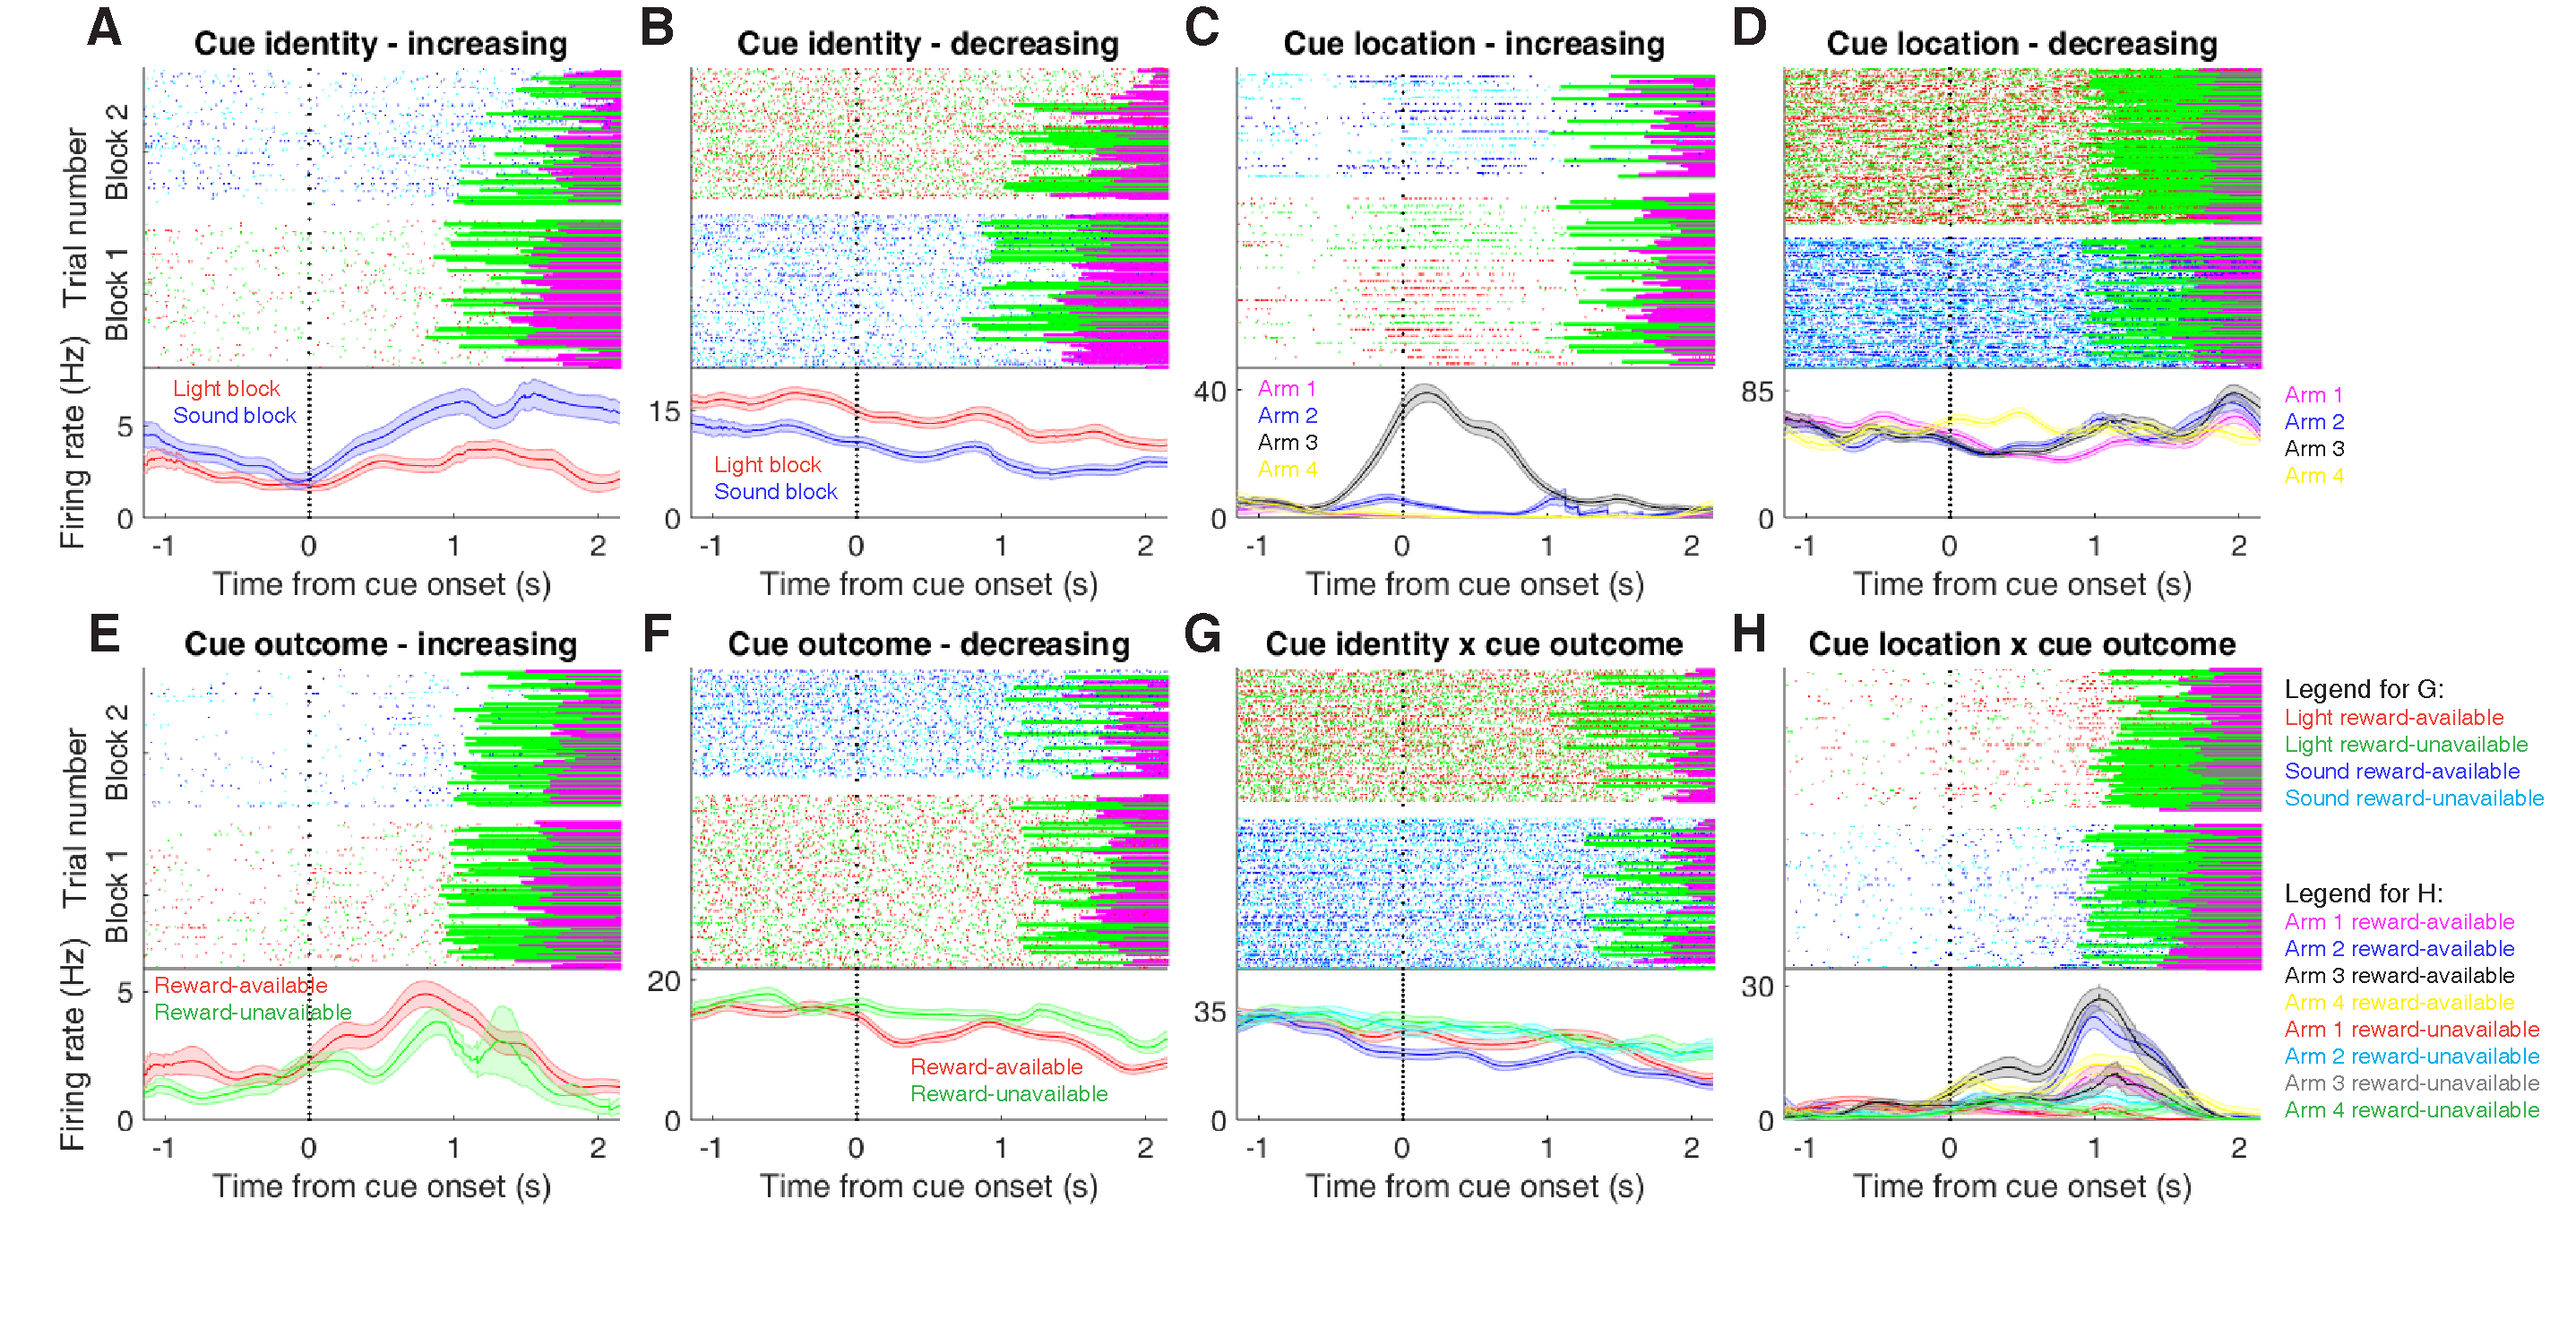
\includegraphics[width=\textwidth]{Fig 5 - Neural examples.pdf}
\caption{Examples of different cue-modulated NAc units influenced by various
  task parameters. \bsf{A}: Example of a cue-modulated NAc unit that showed an
  increase in firing following the cue, and encoded cue identity. Top:
  rasterplot showing the spiking activity across all trials aligned to
  cue-onset. Spikes across trials are color-coded according to cue type (red:
  reward-available light; green: reward-unavailable light; navy blue:
  reward-available sound; light blue: reward-unavailable sound). Green and
  magenta bars indicate trial termination when a rat initiated the next trial or
  made a nosepoke, respectively. White space halfway up the rasterplot indicates
  switching from one block to the next. Dashed line indicates cue onset. Bottom:
  PETHs showing the average smoothed firing rate for the unit for trials during
  light (red) and sound (blue) blocks, aligned to cue-onset. Lightly shaded area
  indicates standard error of the mean. Note this unit showed a larger increase
  in firing to sound cues. \bsf{B}: An example of a unit that was responsive to
  cue identity as in A, but for a unit that showed a decrease in firing to the
  cue. Note the sustained higher firing rate during the light block. \bsf{C-D}:
  Cue-modulated units that encoded cue location, each color in the PETHs
  represents average firing response for a different cue location. \bsf{C}: The
  firing rate of this unit only changed on arm 3 of the task. \bsf{D}: Firing
  decreased for this unit on all arms but arm 4. \bsf{E-F}: Cue-modulated units
  that encoded cue outcome, with the PETHs comparing reward-available (red) and
  reward-unavailable (green) trials. \bsf{E}: This unit showed a slightly higher
  response during presentation of reward-available cues. \bsf{F}: This unit
  showed a dip in firing when presented with reward-available cues. \bsf{G-H}:
  Examples of cue-modulated units that encoded multiple cue features. \bsf{G}:
  This unit integrated cue identity and outcome. \bsf{H}: An example of a unit
  that integrated cue identity and location.}
\label{fig:examples}
\end{figure} \clearpage

 \begin{figure}[ht!]
\centering
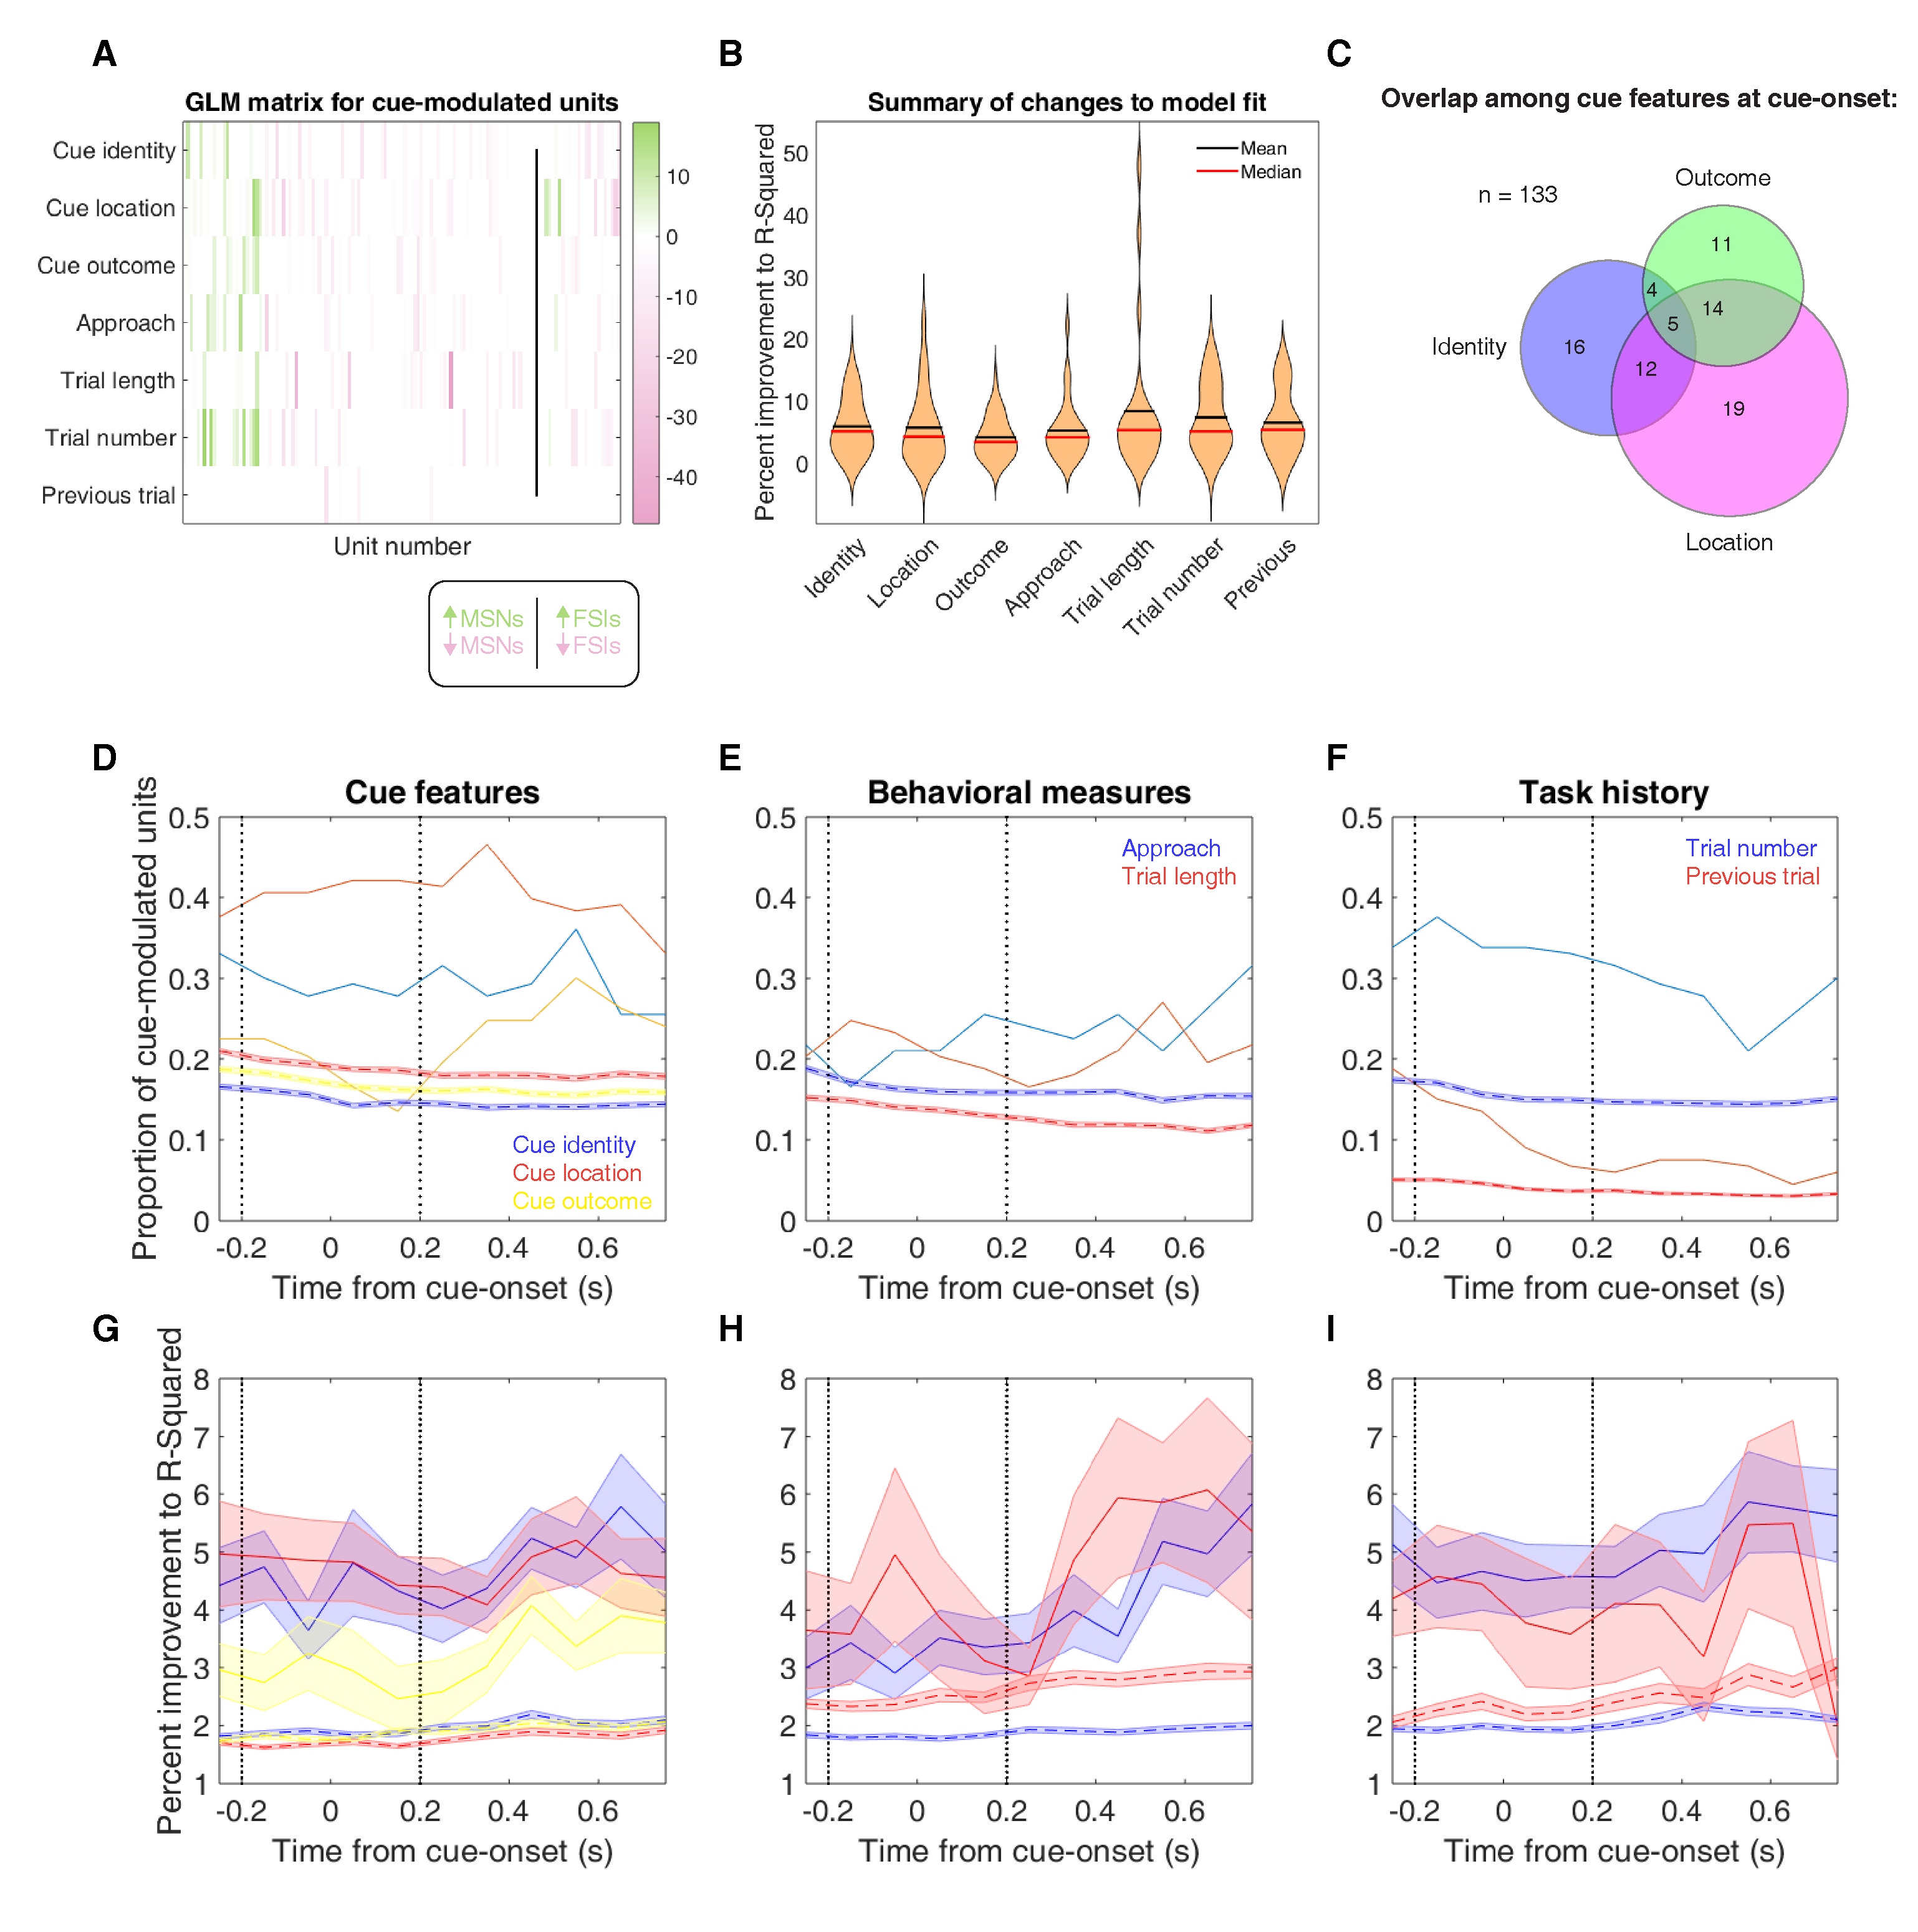
\includegraphics[height=0.5\textheight]{Fig 6 - GLM.pdf}
\caption{Summary of influence of various task parameters on cue-modulated NAc
units after cue-onset. \bsf{A}: GLM matrix illustrating the contribution of
various task parameters to NAc unit firing rates. A stepwise GLM was fit to
each unit that showed evidence of cue modulation by a Wilcoxon signed-rank
test. Each row represents a given task parameter, and each column corresponds
to a single unit. Colors indicate how much of the firing rate variance an
individual predictor contributed to the model, as measured by differences in
R-squared between the final model and the model minus the predictor of
interest. Ordering from left to right: MSNs that increased firing in response
to the cue (green, left of line), MSNs with a decreasing response (red, left
of line), FSIs with an increasing response (green, right of line), FSIs with a
decreasing response (red, right of line). Darker shades indicate more firing
rate variance explained by a given predictor. Black line indicates separation
of MSNs and FSIs. Scale bar indicates range of improvements to model fit for units with an increasing (green) and decreasing (red) response to the cue. \bsf{B}: Violin plots demonstrating changes in R-squared
values with the addition of each of the individual predictors. The mean,
median, and distribution of changes in R-squared values is plotted for each of
the seven task parameters used in the GLM. \bsf{C}: Venn diagram illustrating the number of cue-modulated units encoding cue identity (blue circle), cue location (green circle), cue outcome (pink circle), as well as the overlap among units that encoded multiple cue features. \bsf{D-F}: Sliding window GLM illustrating the proportion of cue-modulated units influenced by various predictors around time of cue-onset. \bsf{D}: Sliding window GLM (bin size: 500 ms; step size: 100 ms) demonstrating the proportion of cue-modulated units where cue identity (blue solid line), cue location (red solid line), and cue outcome (yellow solid line) significantly contributed to the model at various time epochs relative to cue-onset. Dashed colored lines indicate the average of shuffling the firing rate order that went into the GLM 100 times. Points in between the two vertical dashed lines indicate bins where both pre- and post-cue-onset time periods where used in the GLM. \bsf{E}: Same as D, but for approach behavior and trial length. \bsf{F}: Same as D, but for trial number and previous trial. \bsf{G-I}: Average improvement to model fit. \bsf{G}: Average percent improvement to R-squared for units where cue identity, cue location, or cue outcome were significant contributors to the final model for time epochs surrounding cue onset. Shaded area around mean represents the standard error of the mean. \bsf{H}: Same as G, but for approach behavior and trial length. \bsf{I}: Same G, but for trial number and previous trial.}
\label{fig:GLM}
\end{figure} \clearpage

{\bf Population level averages reveal characteristic response profiles:}

We observed a variety of single unit response profiles around the time of cue
onset (Figure \ref{fig:examples}). To investigate whether these firing rate
patterns were related to what cue features were encoded, we plotted the
population level averages for units that were modulated by each feature. To do
this, we normalized firing activity for each unit that was modulated by a given
cue feature, such as light block, then generated the cue-onset aligned
population average firing rate for each of the cue features (Figure
\ref{fig:pop}). Overall, this analysis revealed that cells that showed an
increase upon cue presentation had stronger responses for the preferred cue
condition (Figure \ref{fig:pop}A,C,E). Interestingly, units that were classified
as decreasing in response to the cue showed a biphasic response at the
population level, with a small peak at a time in alignment with entry into the
arm, followed by a sustained dip after cue-onset (Figure
\ref{fig:pop}B,D,F). Units that were modulated by cue identity showed a stronger
increase in response to the preferred task block, as well as a higher tonic
firing rate to the preferred task block, most notably in units that decreased in
firing rate to the cue (Figure \ref{fig:pop}A,B). Units that were modulated by
cue location showed a graded response to locations of decreasing preference,
with peak firing occurring around cue-onset (Figure \ref{fig:pop}C,D). Units
that were modulated by cue outcome showed a ramping of activity after cue-onset
for their preferred cue type. Additionally, units that exhibited a decrease in
firing in response to the cue and whose activity was modulated by cue outcome,
showed a sustained discriminatory response to reward-available and
reward-unavailable cues that extended beyond cue-onset (Figure
\ref{fig:pop}F). Together, these visualizations of the averaged population
responses revealed nuanced differences in the way NAc units are modulated by cue
conditions across cue features.


 \begin{figure}[ht!]
\centering
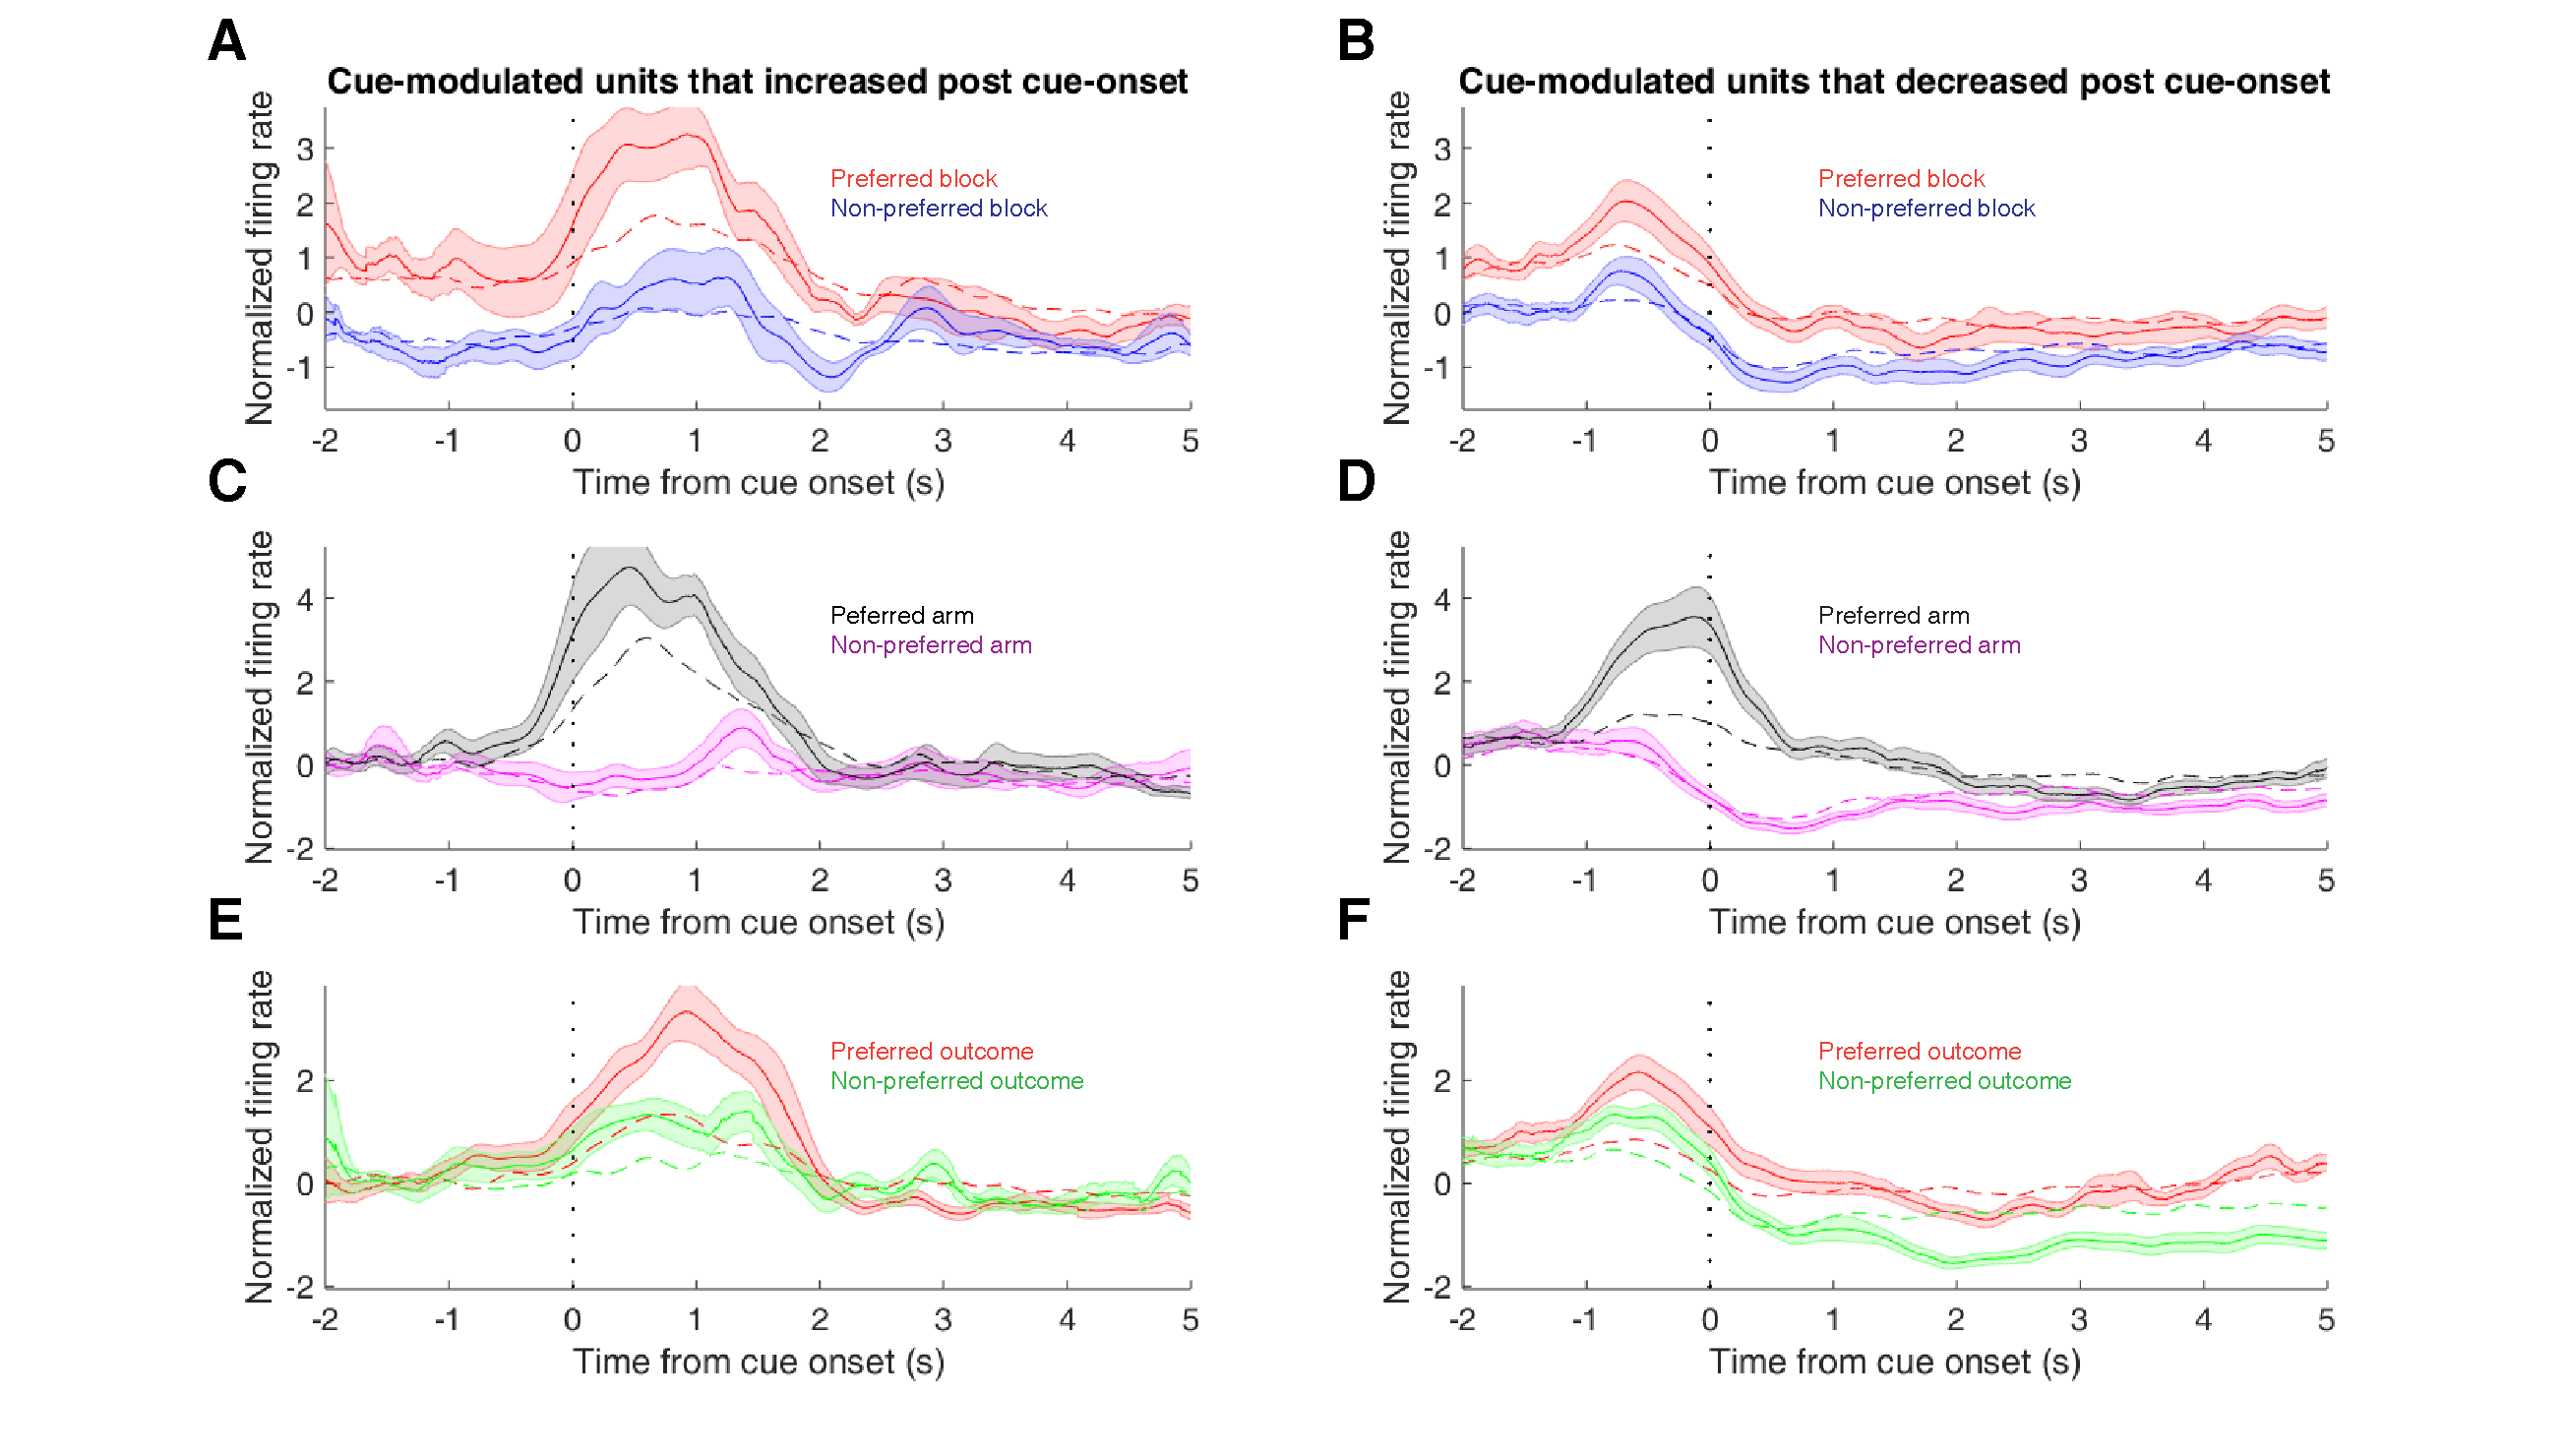
\includegraphics[width=\textwidth]{Fig 7 - Population averages.pdf}
\caption{Population-level averages of cue feature sensitive NAc units. \bsf{A}:
  Average smoothed normalized (z-score) activity for cue-modulated units where
  cue identity was a significant predictor in the GLM, aligned to
  cue-onset. Activity is plotted for preferred stimulus block (red) and
  nonpreferred stimulus block (blue). Dashed vertical line indicates onset of
  cue. Dashed color lines indicate the result of shuffling the identity of the units used for this average 1000 times. Lightly shaded area indicates standard error of the mean. Note larger
  increase to preferred stimulus block over nonpreferred stimulus block. Black
  lines indicate the average of 1000 rounds of random sampling of units from the
  non-drifting population for the preferred and non-preferred blocks. \bsf{B}:
  Same as A but for units that decreased in firing. Note population level
  activity reveals units classified as “decreasing” in response to cue show a
  biphasic response at the population level, with a transient increase around
  the time the rat starts on the arm, followed by a minimum after cue
  onset. Also, note the sustained difference in firing between the two
  blocks. \bsf{C-D}: Same as A-B for cue location. Activity is plotted for
  most preferred arm (black) and least preferred arm (magenta). \bsf{E-F}: Same as A-B for cue outcome. Activity is
  plotted for preferred expected outcome (red), and nonpreferred outcome
  (green). Note the larger increase to the cue representing the unit’s preferred
  outcome (E), and the sustained decrease to the nonpreferred outcome (F).}
\label{fig:pop}
\end{figure} \clearpage

{\bf NAc units dynamically segment the task:}

Given the varied time courses and response profiles of NAc units to various
aspects of the cue, the NAc may be computing a temporally evolving state value
signal (Pennartz., 2011). If this is the case, then the recruitment of NAc units
should vary alongside changes in the environment. To look at the distribution of
responses throughout our task space and see if this distribution is modulated by
cue features, we z-scored the firing rate of each unit and plotted the
normalized firing rates of all units aligned to cue-onset and sorted them
according to the time of peak firing rate (Figure \ref{fig:tiling}). We did this
separately for both the light and sound blocks, and found a nearly uniform
distribution of firing fields in task space that was not limited to alignment to
the cue (Figure \ref{fig:tiling}A). Furthermore, to determine if this population
level activity was similar across blocks, we also organized firing during the
sound blocks according to the ordering derived from the light blocks. This revealed that while there was some preservation of order, the overall firing was qualitatively different
across the two blocks, implying that population activity distinguishes between light and sound blocks. To control for the possibility that any comparison of
trials would produce this effect, we did a within block comparison, comparing
half of the trials in the light block against the other half. This comparison
looked similar to our test comparison of sound block trials ordered by light
block trials. Additionally, given that the majority of our units showed an
inhibitory response to the cue, we also plotted the firing rates according to
the lowest time in firing, and again found some maintenance of order, but
largely different ordering across the two blocks, and the within block
comparison (Figure \ref{fig:tiling}D). To further test this, we divided each
block into two halves and looked at the correlation of the average smoothed
firing rates across various combinations of these halves across our cue-aligned
centered epoch. A linear mixed effects model revealed that within block
correlations (e.g. one half of light trials vs other half of light trials) were
higher and more similar than across block correlations (e.g. half of light
trials vs half of sound trials) suggesting that activity in the NAc
discriminates across various cue conditions (within block correlations = .383 (light), .379 (sound); across block correlations = .343, .338, .337, .348; within block vs.\ within block comparison = p $=$ .934; within block vs.\ across block comparisons = p $<$ .001). This process was repeated for cue location (Figure \ref{fig:tiling}B,E; within block correlations = .369 (arm 1), .350 (arm 2); across block correlations = .290, .286, .285, .291; within block vs.\ within block comparison = p $=$ .071; within block vs.\ across block comparisons = p $<$ .001) and cue outcome (Figure \ref{fig:tiling}C,F;  within block correlations = .429 (reward-available), .261 (reward-unavailable); across block correlations = .258, .253, .255, .249; within block vs.\ within block comparison = p $<$ .001; within block vs.\ across block comparisons = p $<$ .001), showing that NAc segmentation of the task is qualitatively
different even during those parts of the task not immediately associated with a
specific cue, action, or outcome, although the within condition comparison of
reward-unavailable trials was less correlated than reward-available trials, and
more similar to the across condition comparisons, potentially due do the greater behavioral variability for the reward-unavailable trials.

 \begin{figure}[ht!]
\centering
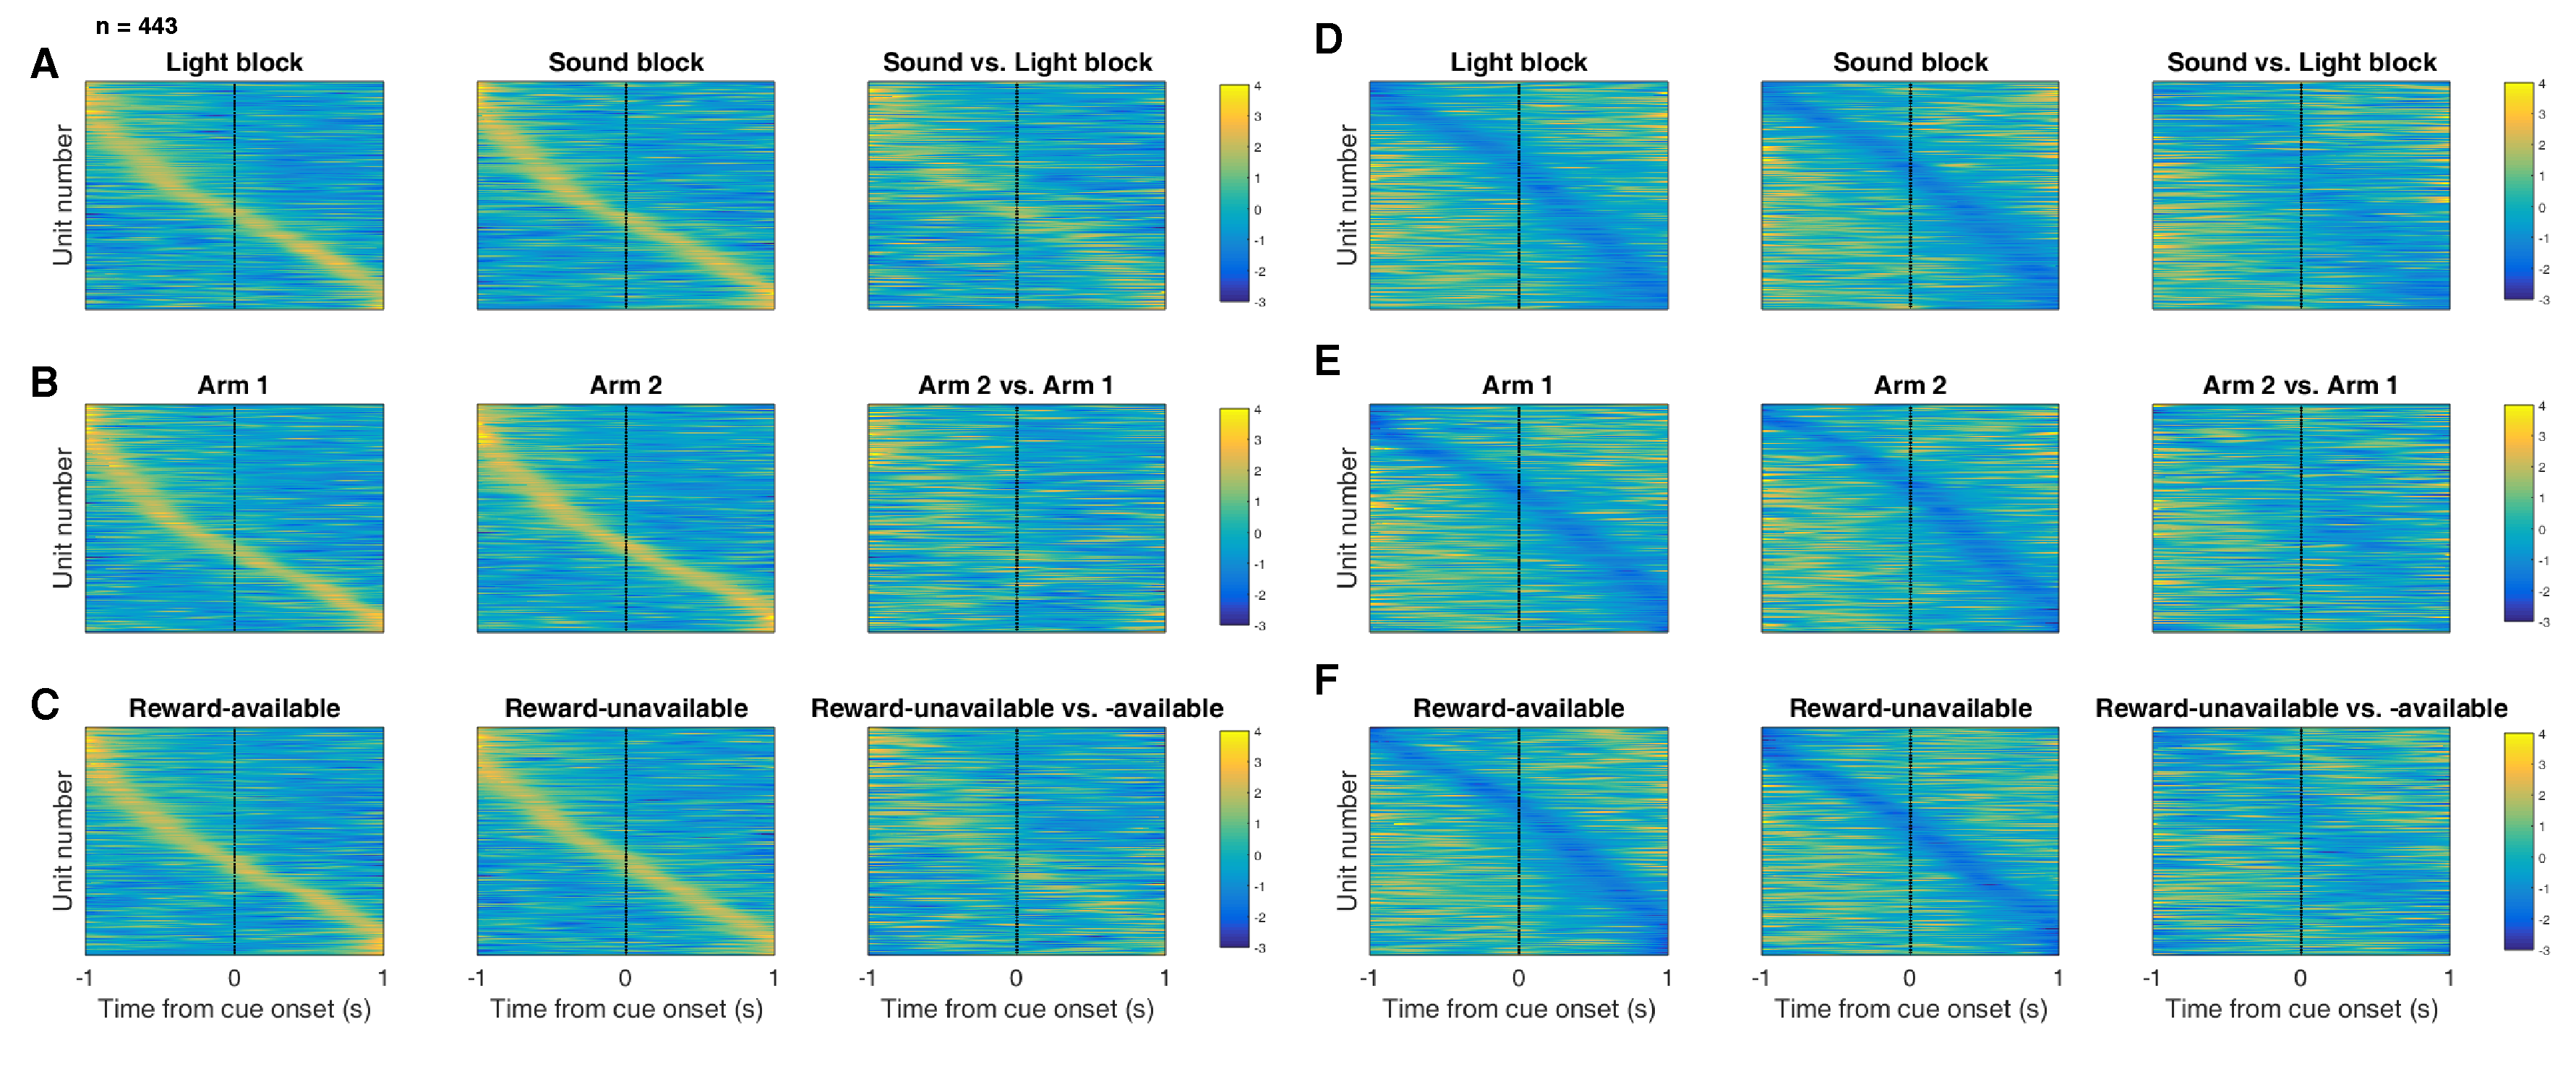
\includegraphics[width=\textwidth]{Fig 8 - Task tiling.pdf}
\caption{Distribution of NAc firing rates across time surrounding cue
onset. Each panel shows normalized (z-score) firing rates for all recorded NAc
units (each row corresponds to one unit) as a function of time (time 0
indicates cue onset), averaged across all trials for a specific cue type,
indicated by text labels. \bsf{A-C}: Heat plots aligned to normalized peak
firing rates. \bsf{A}, left: Heat plot showing smoothed normalized firing
activity of all recorded NAc units ordered according to the time of their peak
firing rate during the light block. Each row is a unit’s average activity
across time to the light block. Dashed line indicates cue onset. Notice the
yellow band across time, indicating all aspects of visualized task space were
captured by the peak firing rates of various units. A, middle: Same units
ordered according to the time of the peak firing rate during the sound
block. Note that for both blocks, units tile time approximately uniformly with
a clear diagonal of elevated firing rates. A, right: Unit firing rates
taken from the sound block, ordered according to peak firing rate taken from
the light block. Note that a weaker but still discernible diagonal persists,
indicating partial similarity between firing rates in the two blocks. A similar pattern exists for within-block comparisons suggesting that reordering any two sets of trials
produces this partial similarity, however correlations within blocks are more
similar than correlations across blocks (see text). \bsf{B}: Same layout as in
A, except that the panels now compare two different locations on the track
instead of two cue modalities. As for the different cue modalities, NAc units
clearly discriminate between locations, but also maintain some similarity
across locations, as evident from the visible diagonal in the right panel. Two
example locations were used for display purposes; other location pairs showed
a similar pattern. \bsf{C}: Same layout as in A, except that panels now
compare reward-available and reward-unavailable trials. \bsf{D-F}: Heat plots
aligned to normalized minimum firing rates. \bsf{D}: Responses during
different stimulus blocks as in A, but with units ordered according to the
time of their minimum firing rate. \bsf{E}: Responses during trials on
different arms as in B, but with units ordered by their minimum firing
rate. \bsf{F}: Responses during cues signalling different outcomes as in C,
but with units ordered by their minimum firing rate. Overall, NAc units
"tiled" experience on the task, as opposed to being confined to specific task
events only. Units from all sessions and animals were pooled for this
analysis.}
\label{fig:tiling}
\end{figure} \clearpage

{\bf Encoding of cue features persists until outcome:}

In order to be useful for credit assignment in reinforcement learning, a trace
of the cue must be maintained until the outcome, so that information about the
outcome can be associated with the outcome-predictive cue. To test whether
representations of cue features persisted post-approach until the outcome
was revealed, we fit a GLM to the post-approach firing rates of cue-modulated
units aligned to the time of nosepoke into the reward receptacle. This analysis
showed that a variety of units still discriminated firing according to various
cue features, but not other task parameters, showing that NAc activity
discriminates various cue conditions well into a trial (Table \ref{tbl1},
Figures \ref{fig:NP_examples},\ref{fig:NP_GLM}). Additionally, these units were
a mix between most of the units that encoded cue features at cue-onset (observed
overlap greater than expected by chance according to chi-square tests), and those
that did not previously have a cue feature as a predictor (29, 48, and 30 out of 133 cue-modulated units encoded both time points for cue identity, cue location, and cue outcome,
respectively). Population level averages for units that increased to
cue-onset showed a ramping up of activity that peaked upon nosepoke, whereas
units that decreased to cue-onset showed a gradual reduction of firing activity
that reached a minimum upon nosepoke (Figure \ref{fig:NP_pop}). Additionally, a
peak is seen for preferred cue outcome in decreasing units at 1 second post
cue-onset when reward was received, demonstrating an integration of expected and
received reward (Figure \ref{fig:NP_pop}F). Furthermore, aligning normalized
peak firing rates to nosepoke onset, revealed a clustering of responses around
outcome receipt for all cue conditions where the rat would have received reward
(Figure \ref{fig:NP_tiling}), in addition to the same trend of higher within- vs across-block correlations for cue identity (Figure \ref{fig:NP_tiling}A,C; within block correlations = .560 (light), .541 (sound); across block correlations = .487, .481, .483, .486; within block vs. within block comparison = p $=$ .112; within block vs. across block comparisons = p $<$ .001) and cue location (Figure \ref{fig:NP_tiling}B,E; within block correlations = .474 (arm 1), .461 (arm 2); across block correlations = .416, .402, .416, .415; within block vs. within block comparison = p $=$ .810; within block vs. across block comparisons = p $<$ .001), but not cue outcome (Figure \ref{fig:NP_tiling}C,F; within block correlations = .620 (reward-available), .401 (reward-unavailable); across block correlations = .418, .414, .390, .408; within block vs. within block comparison = p $<$ .001; within block vs. across block comparisons = p $<$ .001). To determine whether coding of cue features persisted after the outcome was revealed, a GLM was fit to the firing rates of
cue-modulated units at the time of outcome receipt, during which the cue was
still present. Fitting a GLM revealed 10 units (8\%) where cue outcome accounted
for an average of 32\% of firing rate variance (Table \ref{tbl1}, data not
shown). An absence of cue identity or cue location coding at this level of analysis was observed,
but looking at the data more closely with a sliding window GLM revealed that
cue identity, cue location, and cue outcome were encoded throughout time epochs surround cue-onset, nosepoke hold, and outcome receipt,
suggesting that the NAc maintains a representation of these cue features once the rat receives behavioral feedback for its decision (Figure \ref{fig:NP_GLM}E-J).

 \begin{figure}[ht!]
\centering
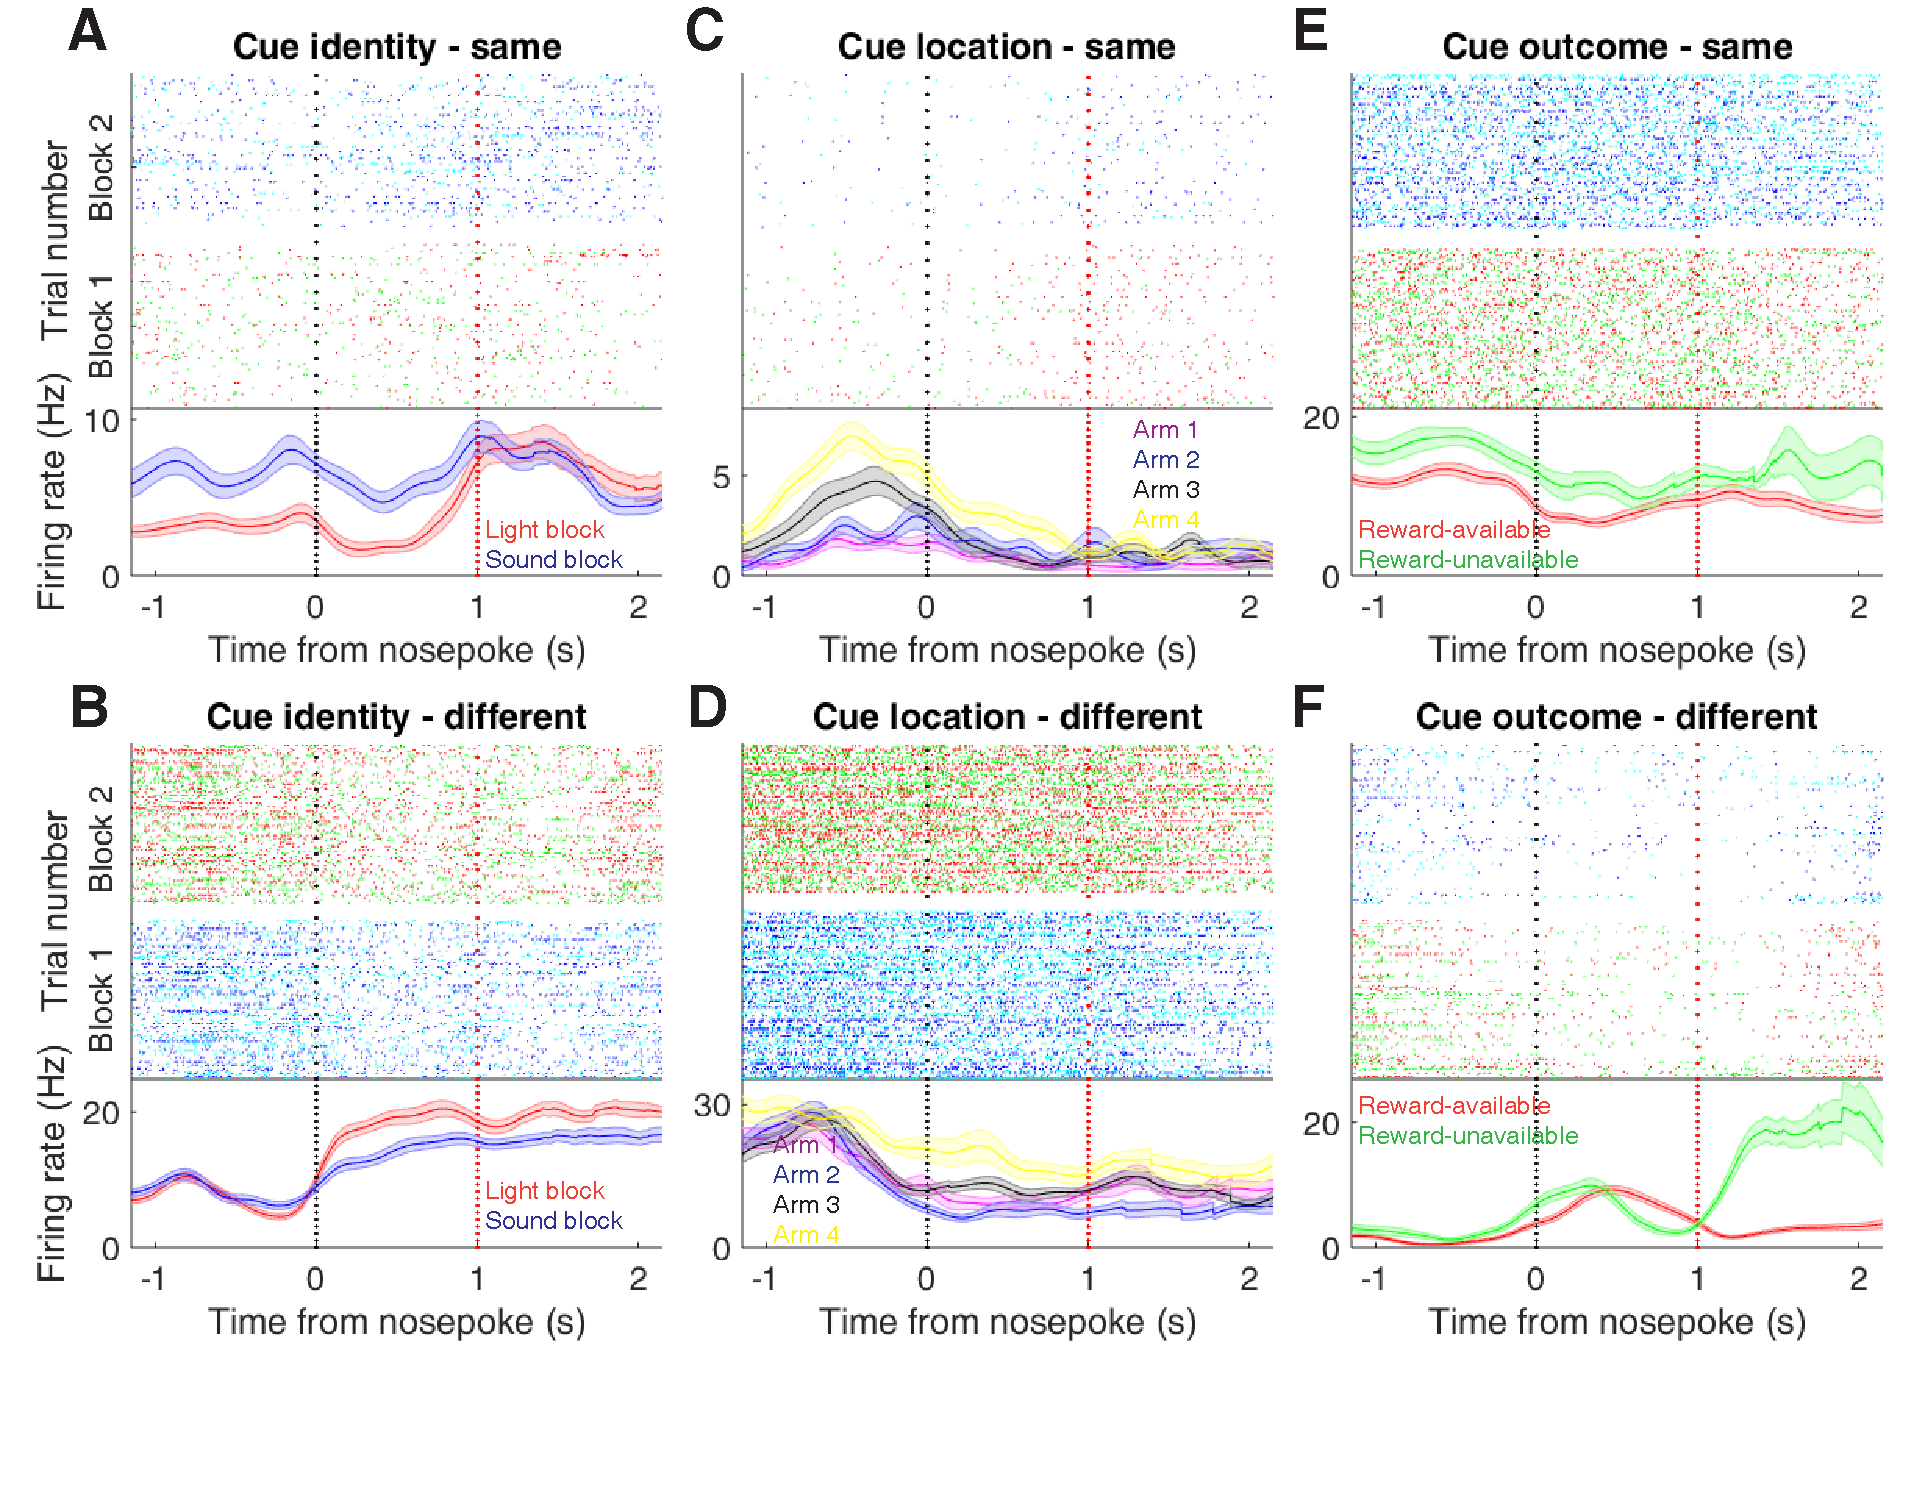
\includegraphics[width=\textwidth]{Fig 9 - NP Neural examples.pdf}
\caption{Examples of cue-modulated NAc units influenced by various task
parameters at time of nosepoke. \bsf{A}: Example of a cue-modulated NAc unit
that encoded cue identity at both cue-onset and during nosepoke hold. Top:
rasterplot showing the spiking activity across all trials aligned to
nosepoke. Spikes across trials are color coded according to cue type (red:
reward-available light; green: reward-unavailable light; navy blue:
reward-available sound; light blue: reward-unavailable sound). White space
halfway up the rasterplot indicates switching from one block to the
next. Black dashed line indicates nosepoke. Red dashed line indicates receipt
of outcome. Bottom: PETHs showing the average smoothed firing rate for the
unit for trials during light (red) and sound (blue) blocks, aligned to
nosepoke. Lightly shaded area indicates standard error of the mean. Note this
unit showed a sustained increase in firing to sound cues during the trial. \bsf{B}: An
example of a unit that was responsive to cue identity at time of nosepoke but
not cue-onset. \bsf{C-D}: Cue-modulated units that encoded cue location, at
both cue-onset and nosepoke (C), and only nosepoke (D). Each color in the
PETHs represents average firing response for a different cue
location. \bsf{E-F}: Cue-modulated units that encoded cue outcome, at both
cue-onset and nosepoke (E), and only nosepoke (F), with the PETHs comparing
reward-available (red) and reward-unavailable (green) trials.}
\label{fig:NP_examples}
\end{figure} \clearpage

 \begin{figure}[ht!]
\centering
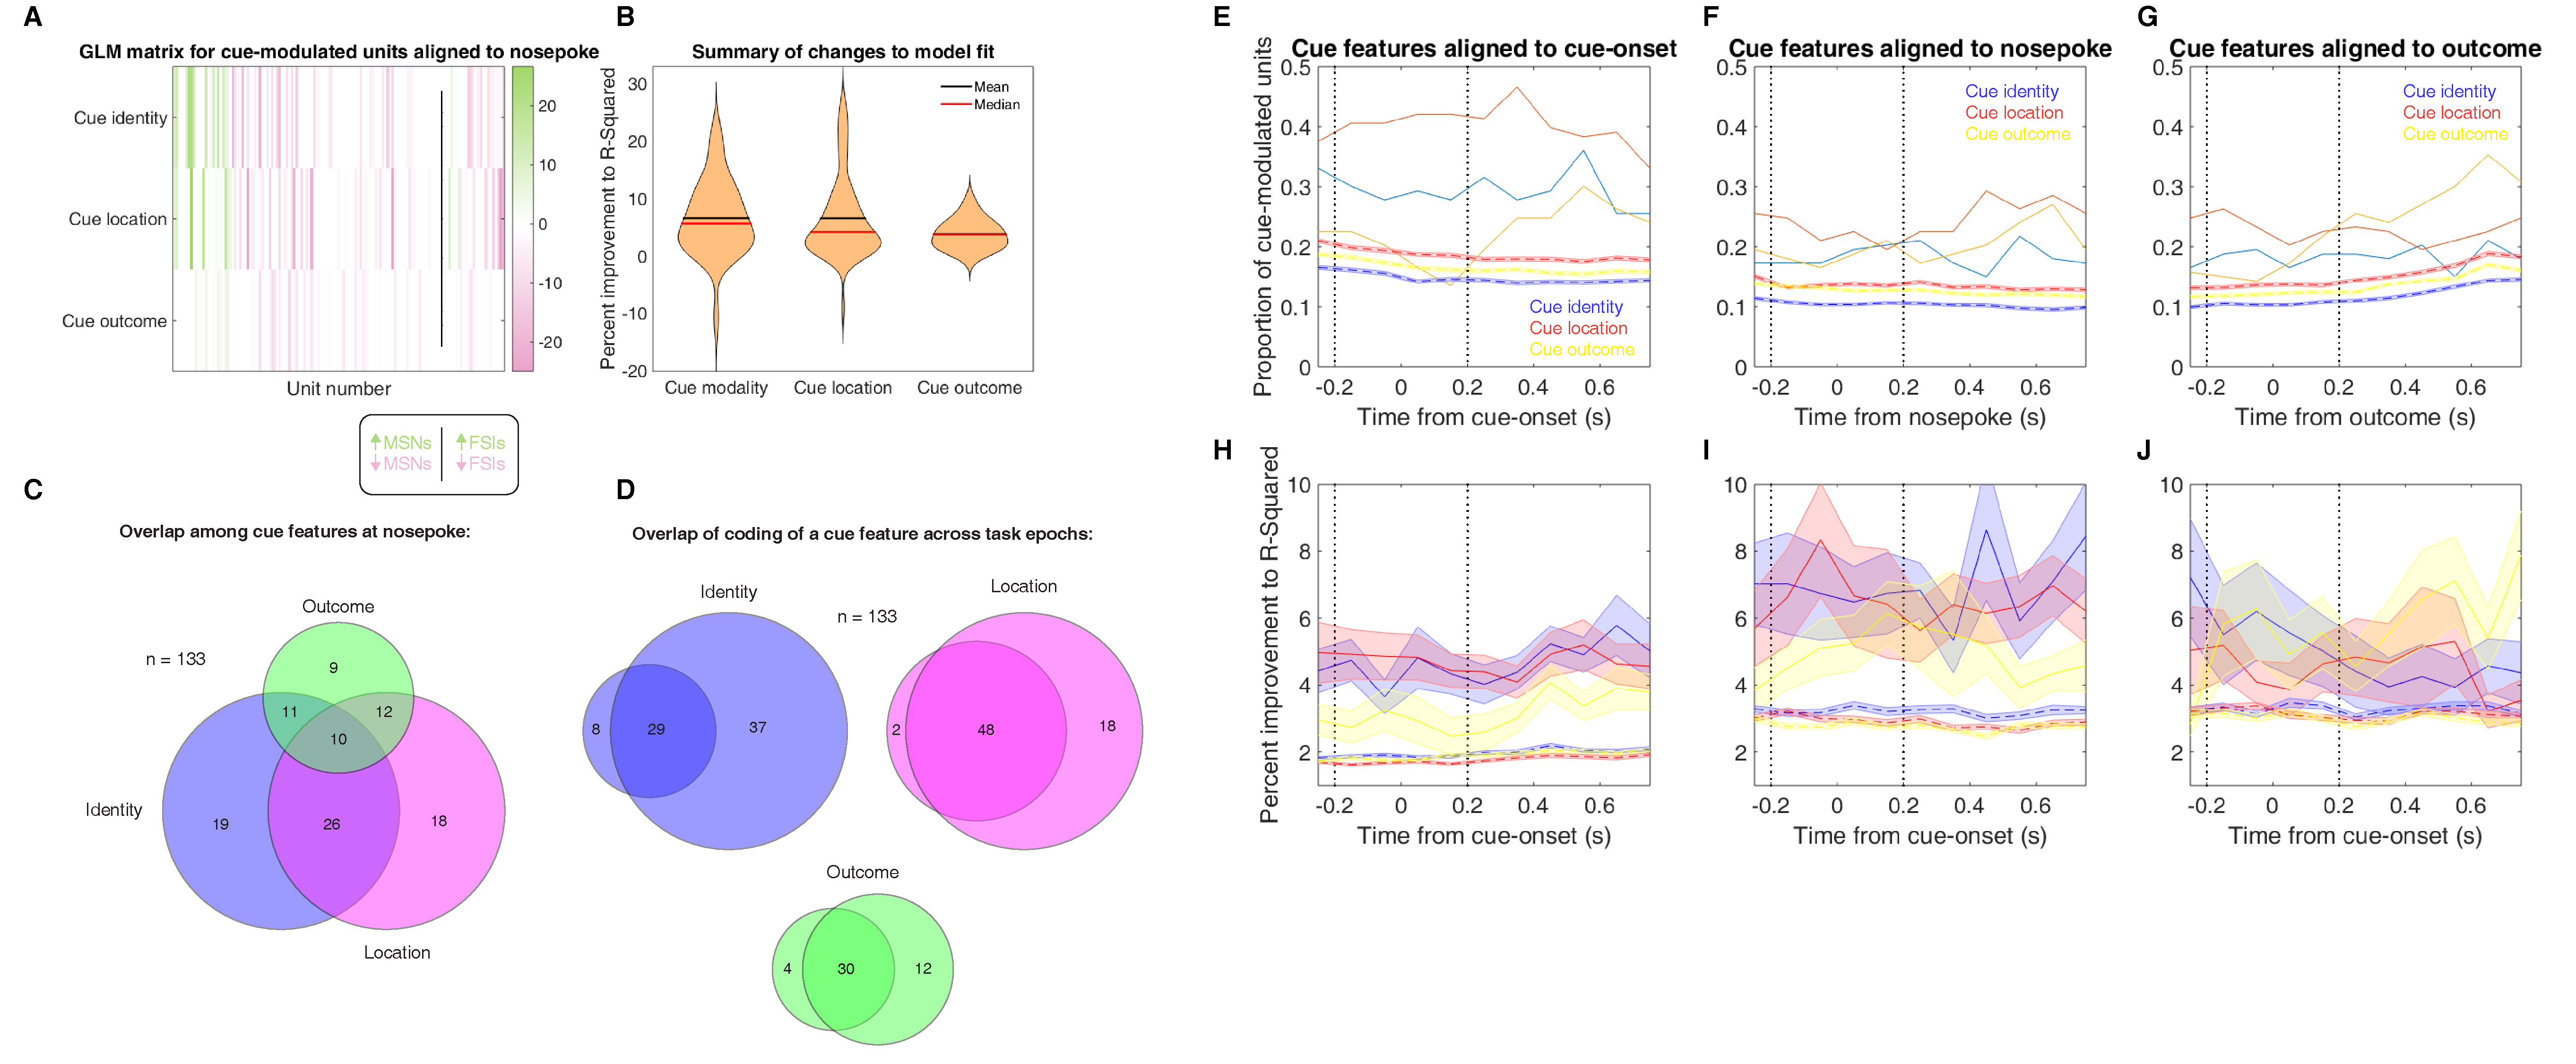
\includegraphics[width=\textwidth]{Fig 10 - NP GLM.pdf}
\caption{Summary of influence of various task parameters on cue-modulated NAc
units during nosepoke. \bsf{A}: GLM matrix illustrating the contribution of various
task parameters to NAc unit firing rates. A stepwise GLM was fit to each unit that
showed evidence of cue modulation by a Wilcoxon signed-rank test. Each row
represents a given task parameter, and each column corresponds to a single unit. Colors indicate how much of the firing rate variance an
individual predictor contributed to the model, as measured by differences in
R-squared between the final model and the model minus the predictor of
Interest. Ordering from left to right: MSNs that increased firing
in response to the cue (green, left of line), MSNs with a decreasing response
(red, left of line), FSIs with an increasing response (green, right of line),
FSIs with a decreasing response (red, right of line). Darker shades indicate
more firing rate variance explained by a given predictor. Black line indicates
separation of MSNs and FSIs. \bsf{B}: Violin plots demonstrating changes in
R-squared values with the addition of each of the individual predictors. The
mean, median, and distribution of changes in R-squared values is plotted for
each of the three task parameters that were significant predictors in the
GLM. \bsf{C}: Venn diagram illustrating the number of cue-modulated units encoding cue identity (blue circle), cue location (green circle), cue outcome (pink circle), as well as the overlap among units that encoded multiple cue features. \bsf{D}: Venn diagram illustrating the number of cue-modulated units encoding cue identity, cue location, and cue outcome during cue-onset (left circle), during nosepoke hold (right circle), and during both epochs (overlap). \bsf{E-G}: Sliding window GLM illustrating the proportion of cue-modulated units influenced by various predictors around time of cue-onset (E), nosepoke (F), and outcome (G). \bsf{E}: Sliding window GLM (bin size: 500 ms; step size: 100 ms) demonstrating the proportion of cue-modulated units where cue identity (blue solid line), cue location (red solid line), and cue outcome (yellow solid line) significantly contributed to the model at various time epochs relative to cue-onset. Dashed colored lines indicate the average of shuffling the firing rate order that went into the GLM 100 times. Points in between the two vertical dashed lines indicate bins where both pre- and post-cue-onset time periods where used in the GLM. \bsf{F}: Same as E, but for time epochs relative to nosepoke where the rat waited for the outcome. \bsf{G}: Same as E, but for time epochs relative to receipt of outcome after the rat got feedback about his approach. \bsf{H-J}: Average improvement to model fit. \bsf{H}: Average percent improvement to R-squared for units where cue identity, cue location, or cue outcome were significant contributors to the final model for time epochs relative to cue-onset. Shaded area around mean represents the standard error of the mean. \bsf{I}: Same as H, but for time epochs relative to nosepoke. \bsf{J}: Same H, but for time epochs relative to receipt of outcome.}
\label{fig:NP_GLM}
\end{figure} \clearpage

 \begin{figure}[ht!]
\centering
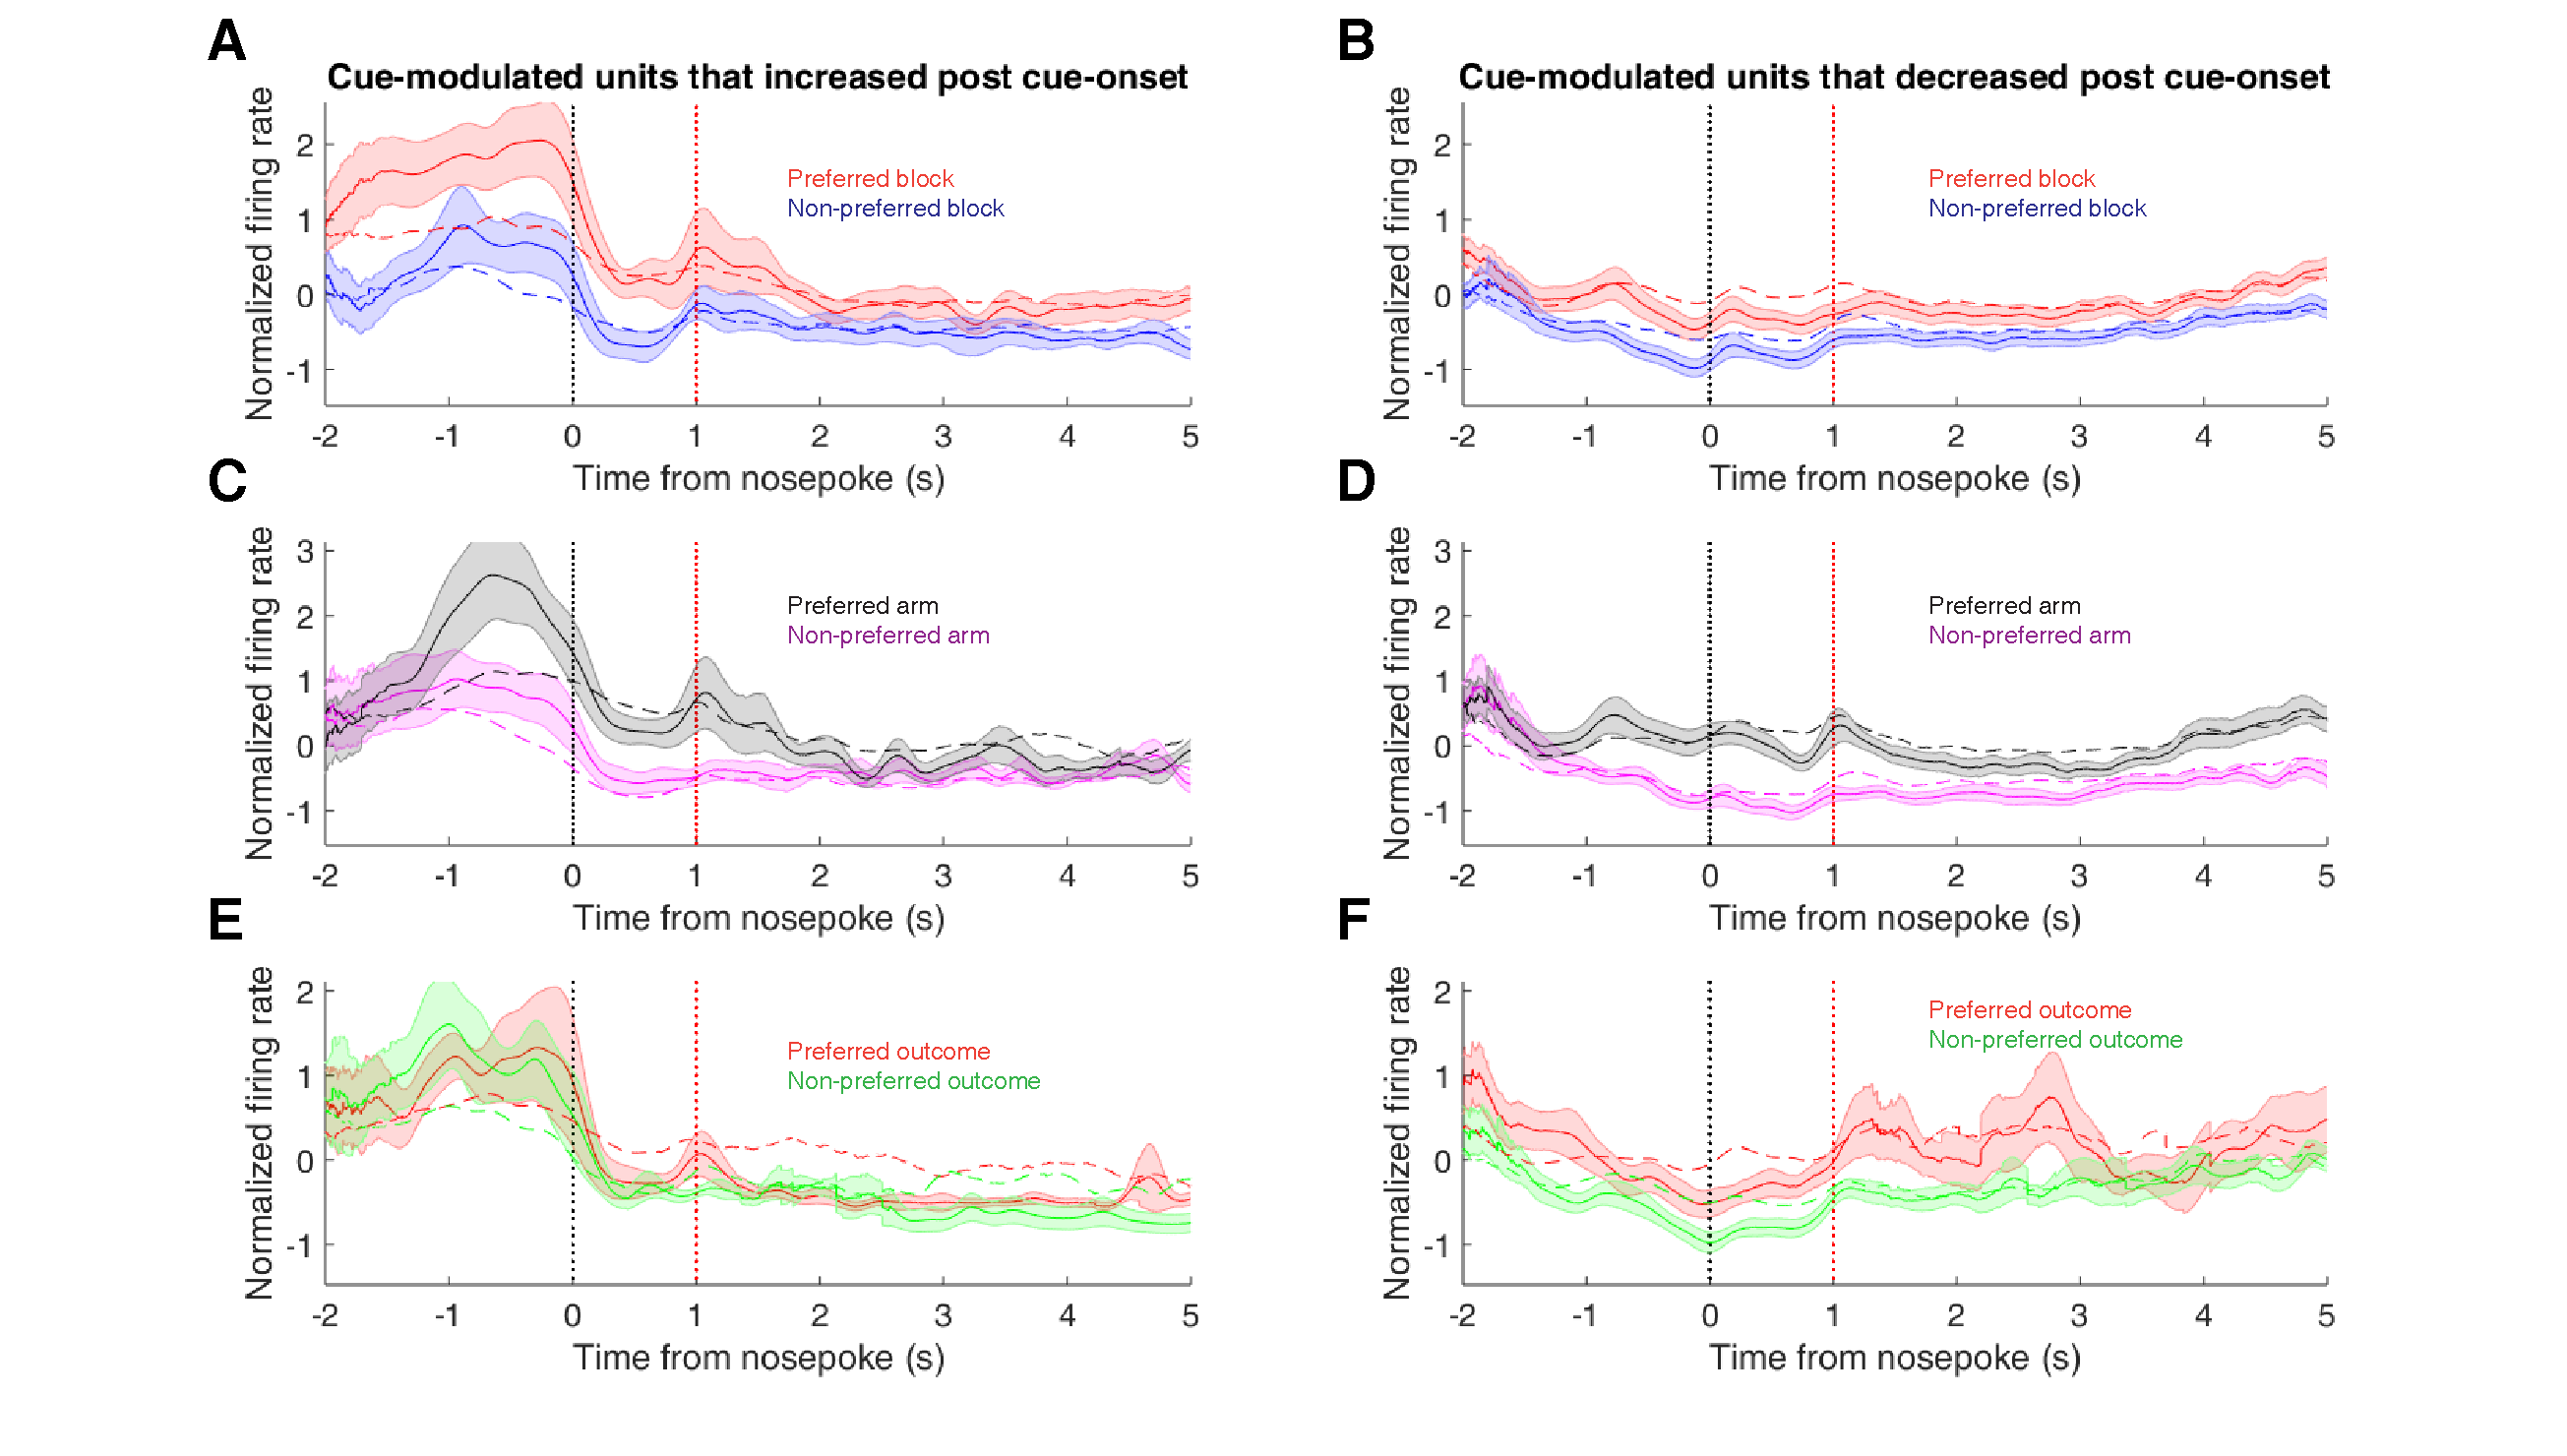
\includegraphics[width=\textwidth]{Fig 11 - NP population averages.pdf}
\caption{Population-level averages of cue feature sensitive NAc units during a
  nosepoke. \bsf{A}: Average smoothed normalized (z-score) activity for cue-modulated
  units where cue identity was a significant predictor in the GLM, aligned to
  nosepoke with reward delivery occurring 1 s after nosepoke. Activity is
  plotted for preferred stimulus block (red) and nonpreferred stimulus block
  (blue). Black vertical dashed line indicates nosepoke. Red vertical dashed line indicates reward
  delivery occurring 1 s after nosepoke for reward-available trials. Dashed color lines indicate the result of shuffling the identity of the units used for this average 1000 times. Lightly
  shaded area indicates standard error of the mean. Note larger increase leading
  up to nosepoke to preferred stimulus block over nonpreferred stimulus
  block. \bsf{B}: Same as A but for units that decreased in firing. Note the
  sustained difference in firing between the two blocks. \bsf{C-D}: Same as A-B
  for cue location. Activity is plotted for most preferred arm (black) and least preferred arm (magneta). \bsf{E-F}: Same as A-B for cue outcome. Activity is plotted for
  preferred expected outcome (red), and nonpreferred outcome (green). Note the
  peak after outcome receipt for preferred outcome in decreasing units (F).}
\label{fig:NP_pop}
\end{figure} \clearpage

 \begin{figure}[ht!]
\centering
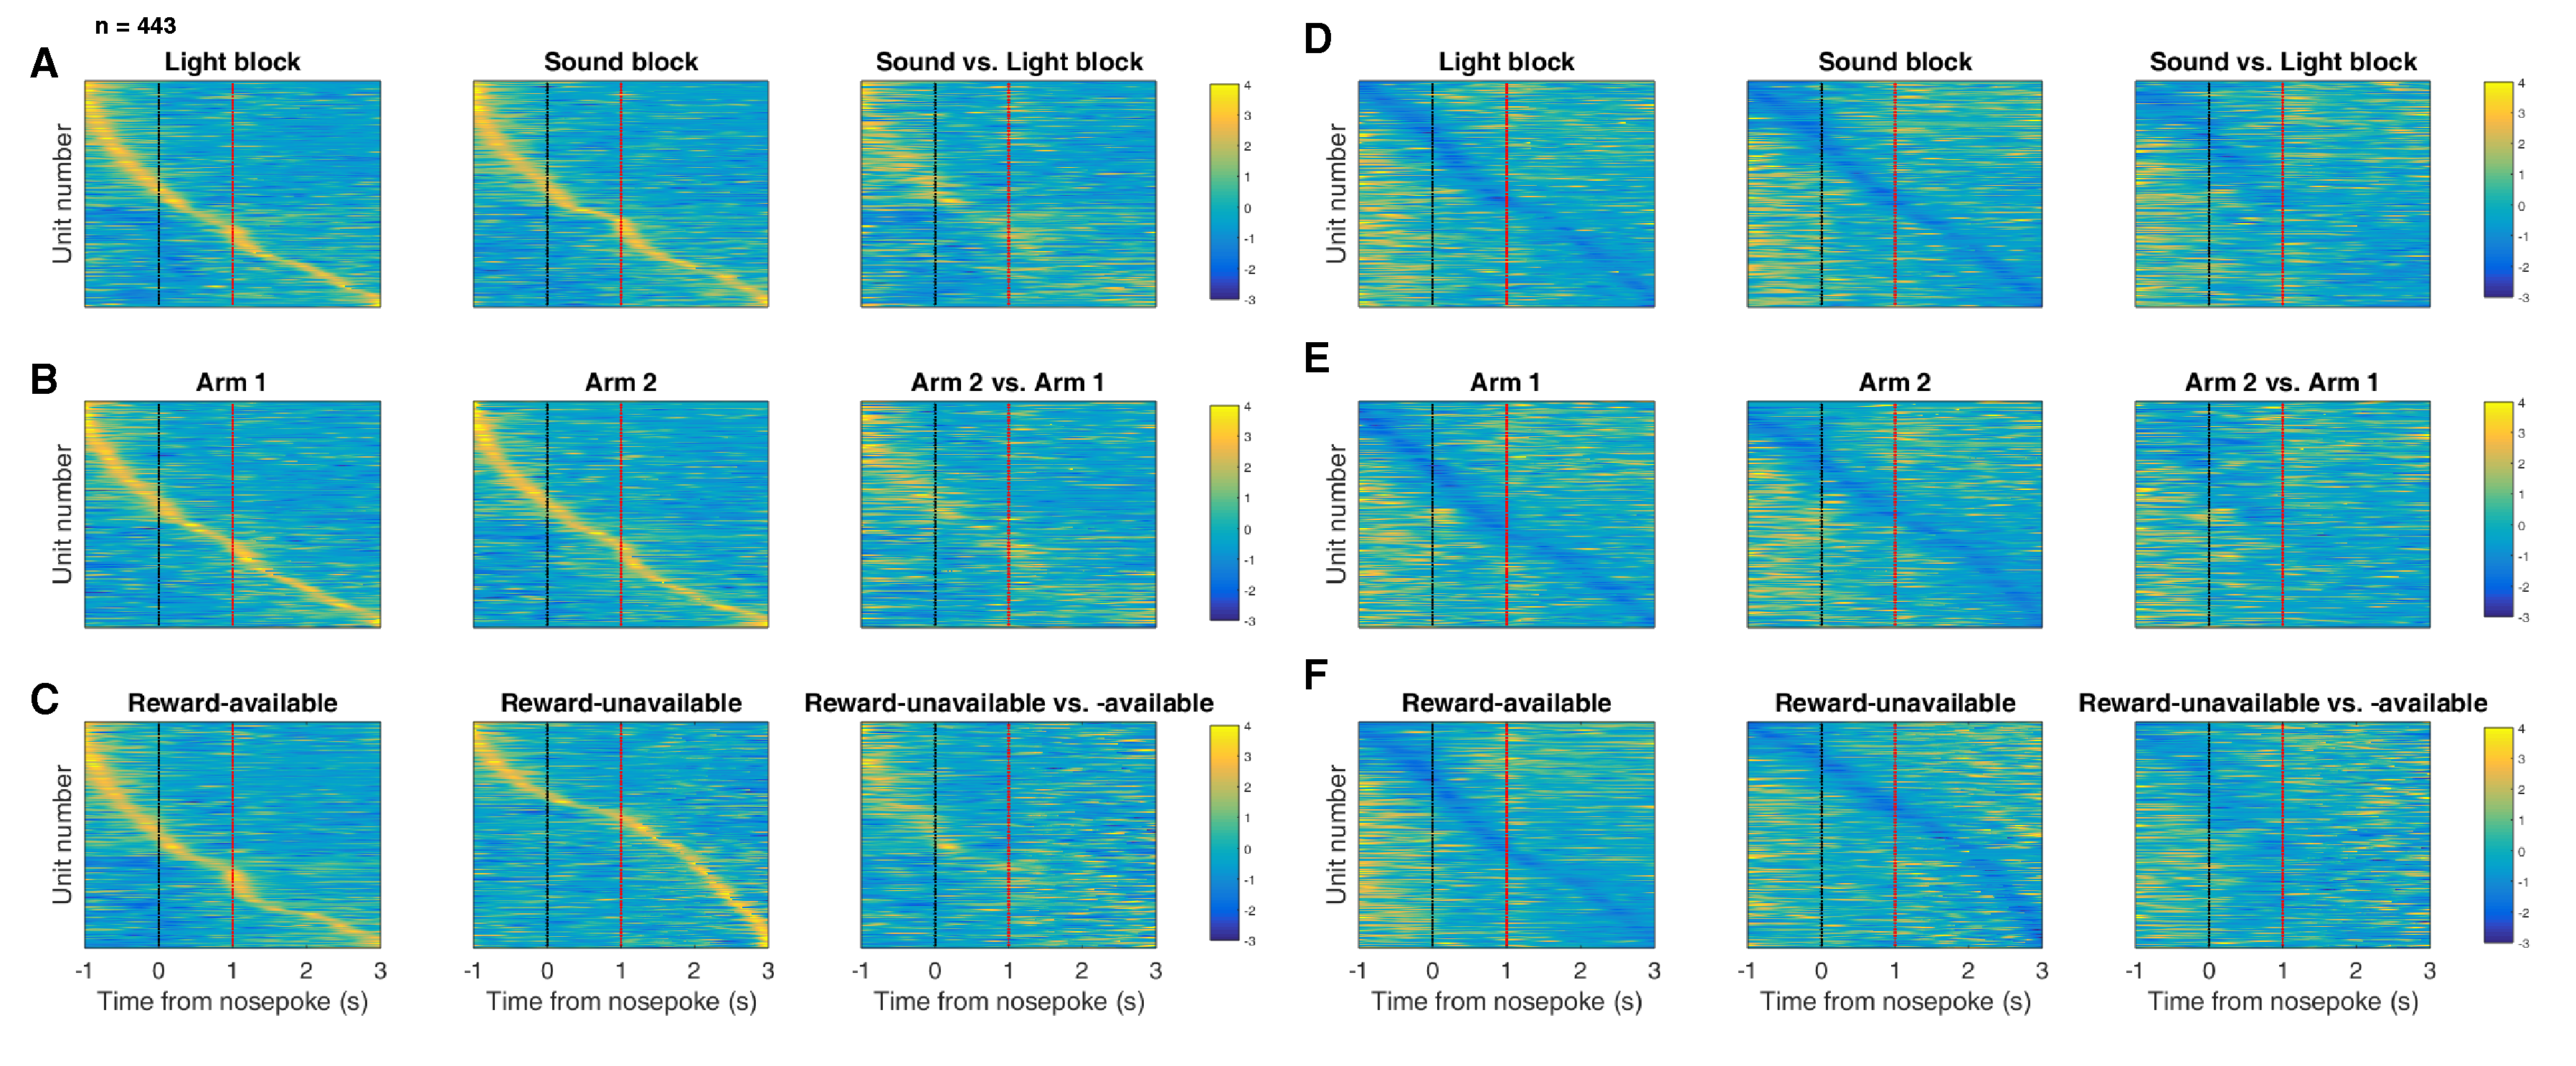
\includegraphics[width=\textwidth]{Fig 12 - NP task tiling.pdf}
\caption{Distribution of NAc firing rates across time surrounding nosepoke for approach
trials. Each panel shows normalized (z-score) firing rates for all recorded NAc units
(each row corresponds to one unit) as a function of time (time 0 indicates
nosepoke), averaged across all approach trials for a specific cue type,
indicated by text labels. \bsf{A-C}: Heat plots aligned to normalized peak firing rates. \bsf{A}, far left: Heat plot showing smoothed
normalized firing activity of all recorded NAc units ordered according to the
time of their peak firing rate during the light block. Each row is a unit’s
average activity across time to the light block. Black dashed line indicates
nosepoke. Red dashed line indicates reward delivery occurring 1 s after
nosepoke for reward-available trials. Notice the yellow band across time,
indicating all aspects of visualized task space were captured by the peak
firing rates of various units. A, middle: Same units ordered according to
the time of the peak firing rate during the sound block. Note that for both
blocks, units tile time approximately uniformly with a clear diagonal of
elevated firing rates, and a clustering around outcome receipt. A, right: Unit firing rates taken from the sound block, ordered according to peak
firing rate taken from the light block. Note that a weaker but still
discernible diagonal persists, indicating partial similarity between firing
rates in the two blocks. A similar pattern exists for within-block comparisons suggesting that
reordering any two sets of trials produces this partial similarity, however
correlations within blocks are more similar than correlations across blocks
(see text). \bsf{B}: Same layout as in A, except
that the panels now compare two different locations on the track instead of
two cue modalities. As for the different cue modalities, NAc units clearly
discriminate between locations, but also maintain some similarity across
locations, as evident from the visible diagonal in the right panel. Two
example locations were used for display purposes; other location pairs showed
a similar pattern. \bsf{C}: Same layout as in A, except that panels now compare
correct reward-available and incorrect reward-unavailable trials. The disproportionate tiling around outcome receipt for reward-available, but not reward-unavailable
trials suggests encoding of reward receipt by NAc units. \bsf{D-F}: Heat plots aligned to normalized minimum firing rates. \bsf{D}: Responses during different stimulus blocks as in A, but with units ordered according to
the time of their minimum firing rate. \bsf{E}: Responses during trials on different arms as in B, but with units ordered by their minimum
firing rate. \bsf{F}: Responses during cues signalling different outcomes as in C, but with units ordered by their minimum firing
rate. Overall, NAc units "tiled" experience on the task, as opposed to being
confined to specific task events only. Units from all sessions and animals
were pooled for this analysis.}
\label{fig:NP_tiling}
\end{figure} \clearpage

\section*{Discussion}

The main result of the present study is that NAc units encode not
only the expected outcome of outcome-predictive cues, but also the
identity of such cues. Importantly, this identity coding was
maintained on approach trials both during a delay period where the rat held
a nosepoke until the outcome was received, after immediately after outcome receipt (H2 and H3 in Figure
\ref{fig:schematic}B). Units coding for cue identity showed partial
overlap with those coding for expected outcome (H3 in Figure
\ref{fig:schematic}A). Units that coded different cue features
(identity, outcome, location) exhibited different temporal profiles as
a whole, although across all recorded units a tiling of task structure
was observed such that all points within our analyzed task space was
accounted for by the ordered peak firing rates of all
units. Furthermore, this tiling differed between various conditions
with a cue feature, such as light versus sound blocks. We discuss
these observations and their implications below.

{\bf Cue identity:}

Our finding that NAc units can discriminate between different
outcome-predictive stimuli with similar motivational significance
(i.e.\ encodes cue identity) expands upon an extensive rodent
literature examining NAc correlates of conditioned stimuli
\cite{Setlow2003,Nicola2004,Yun2004,Roitman2005,Day2006,Ambroggi2008,Ishikawa2008,Roesch2009a,Saddoris2011,Goldstein2012,Lansink2012,Bissonette2013,McGinty2013,Atallah2014,Sugam2014,Cooch2015,West2016,Dejean2017}. Perhaps
the most comparable work in rodents comes from a study that found
distinct coding for an odor when it predicted separate but equally
valued rewards \cite{Cooch2015}. The present work is complementary to
such {\it outcome identity} coding as it shows that NAc units encode {\it cue
  identity}, both separately and integrated with the reward it
predicts (H2 and H3 in Figure \ref{fig:schematic}A). Similarly,
\citeauthor{Setlow2003} (2003) paired distinct cues with appetitive or aversive
outcomes, and found separate populations of units that encoded each
cue. Once again, our study was different in asking how distinct cues
encoding the same anticipated outcome are encoded. Such cue identity
encoding suggests that even when the biological relevance of these
stimuli is similar, NAc dissociates their representations at the level
of the single-units. A possible interpretation of this coding of cue
features alongside expected outcome is that these representations are
used to associate reward with relevant features of the environment,
so-called credit assignment in the reinforcement learning literature
\cite{sutton1998}. A burgeoning body of human and non-human primate
work has started to elucidated neural correlates of credit assignment
in the PFC, particularly in the lateral orbitofrontal cortex
\cite{Chau2015,Akaishi2016,Asaad2017,Noonan2017}. Given the importance
of cortical inputs in NAc associative representations, it is possible
that information related to credit assignment is relayed from the
cortex to NAc \cite{Ishikawa2008,Cooch2015}.

A different possible function for cue identity coding is to support
contextual modulation of the motivational relevance of specific
cues. A context can be understood as a particular mapping between
specific cues and their outcomes: for instance, in context 1 cue A but
not cue B is rewarded, whereas in context 2 cue B but not cue A is
rewarded. Successfully implementing such contextual mappings requires
representation of the cue identities. Indeed, \citeauthor{Sleezer2016} (2016)
recorded NAc responses during the Wisconsin Card Sorting Task,
a common set-shifting task used in both the laboratory and clinic, and
found units that preferred firing to stimuli when a certain rule, or
rule category was currently active. Further support for a
modulation of NAc responses by strategy comes from an fMRI study that
examined BOLD levels during a set-shifting task
\cite{Fitzgerald2014}. In this task, participants learned two sets of
stimulus-outcome contingencies, a visual set and an auditory set. During
testing they were presented with both simultaneously, and the stimulus
dimension that was relevant was periodically shifted between the
two. Here, they found that bilateral NAc activity reflected value
representations for the currently relevant stimulus dimension, and not
the irrelevant stimulus. The current finding of separate, but
overlapping, populations of units encoding cue identity and expected
outcome, suggests that the fMRI finding is generated by the combined
activity of several different functional cell types.

Our analyses were designed to eliminate several potential alternative
interpretations to cue identity coding. Because the different cues
were separated into different blocks, units that discriminated between
cue identities could instead be encoding time or other slowly-changing
quantities. We excluded this possible confound by excluding units that
showed a drift in firing between the first and second half within a
block. However, the possiblity remains that instead of or in addition
to stimulus identity, these units encode a preferred context, or even
a macroscale representation of progress through the session. Indeed,
encoding of the current strategy could be an explanation for the
sustained difference in population averaged firing across stimulus
blocks (Figure \ref{fig:pop}), as well as a potential explanation for
the differentially tiling of task structure across blocks in the
current study (Figure \ref{fig:tiling}).

A different potential confound is that between outcome and action
value coding. We discriminated between these possiblities by analzying
error trials, where the rat appraoched reward (left turn) after
presentation of the reward-unavailable cue. Units that were modulated
by the expected outcome of the cue maintained their specific firing
patterns even during error trials, as expected from outcome value
coding but not action value coding. Additionally, NAc signals have
been shown to be modulated by response vigor \cite{McGinty2013}; to
detangle this from our results we included trial length (i.e.\ latency
to arrival at the reward site) as a predictor in our GLMs, and found
units with cue feature correlates independent of trial length.

An overall limitation of the current study is that rats were never
presented with both sets of cues simultaneously, and were not required
to switch strategies between multiple sets of cues. Thus, it is
unknown to what extent the cue identity encoding we observed is
behaviorally relevant, although extrapolating data from other work
\cite{Sleezer2016} suggests that cue identity coding would be
modulated by relevance. NAc core lesions have been shown to impair
shifting between different behavioral strategies \cite{Floresco2006a},
and it is possible that selectively silencing the units that prefer
responding for a given modality or rule would impair performance when
the animal is required to use that information, or artificial
enhancement of those units would cause them to use the rule when it is
the inappropriate strategy.

{\bf Encoding of position:}

Our finding that cue-evoked activity was modulated by cue location is
in alignment with several previous reports
\cite{Lavoie1994,Wiener2003,Mulder2005,Strait2016}. The NAc receives
inputs from the hippocampus, and the communication of place-reward
information across the two structures suggests that the NAc tracks
locations associated with reward
\cite{Tabuchi2000,Pennartz2004,Lansink2008,Lansink2009,VanderMeer2011,Lansink2016,Sjulson2017}. NAc
units can also signal progress through a sequence of cues and/or
actions
\cite{Shidara1998,Mulder2004,Khamassi2008,Berke2009,Lansink2012,Atallah2014}. Given
that the current task was pseudo-random, it is possible that the rats
learned the structure of sequential cue presentation, and the neural
activity could reflect this. However, this is unlikely as including a
‘previous trial’ variable in the analysis did not explain a
significant amount of firing rate variance in response to the cue for
the vast majority of units. In any case, NAc units on the present
task continued to distinguish between different locations, even though
location, and progress through a sequence, were explicitly irrelevant
in predicting reward. We speculate that this persistent coding of
location in NAc may represent a bias in credit assignment, and
associated tendency for rodents to associate motivationally relevant
events with the locations where they occur.

{\bf Implications:}

Maladaptive decision making, as occurs in schizophrenia, addiction,
Parkinson's, among others, can result from dysfunctional RPE and value
signals \cite{Frank2004,Gradin2011,Maia2011}. This view has been
successful in explaining both positive and negative symptoms in
schizophrenia, and deficits in learning from feedback in Parkinson's
\cite{Frank2004,Gradin2011}. However, the effects of RPE and value
updating are contingent upon encoding of preceding action and cue
features, the eligibility trace \cite{sutton1998,Lee2012}. Value
updates can only be performed on these aspects of preceding experience
that are encoded when the update occurs. Therefore, maladaptive
learning and decision making can result from not only aberrant RPEs
but also from altered cue feature encoding. For instance, on this task
the environmental stimulus that signaled the availability of reward
was conveyed by two distinct cues that were presented in four
locations. While in our current study, the location and identity of
the cue did not require any adjustments in the animal’s behavior, we
found coding of these features alongside the expected outcome of the
cue that could be the outcome of credit assignment computations
computed upstream. Identifying neural coding related to an aspect of
credit assignment is important as inappropriate credit assignment
could be a contributor to conditioned fear overgeneralization seen in
disorders with pathological anxiety such as generalized anxiety
disorder, post traumatic stress disorder, and obsessive-compulsive
disorder \cite{Kaczkurkin2013,Lissek2014,Kaczkurkin2017}, and
delusions observed in disorders such as schizophrenia, Alzheimer's and
Parkinson's \cite{Kapur2003,Corlett2010}. Thus, our results provide a
neural window into the process of credit assignment, such that the
extent and specific manner in which this process fails in syndromes such as schizophrenia, obsessive-compulsive disorder,
etc.\ can be experimentally accessed.

\section*{Methods}

{\bf Subjects:}

A sample size of 4 adult male Long-Evans rats (Charles River, Saint Constant, QC) from an apriori determined sample of 5 
were used as subjects (1 rat was excluded from the data set due to poor cell yield). Rats were individually housed with a 12/12-h
light-dark cycle, and tested during the light cycle. Rats were food
deprived to 85-90\% of their free feeding weight (weight at time of
implantation was 440 - 470 g), and water restricted 4-6 hours before
testing. All experimental procedures were approved by the the
University of Waterloo Animal Care Committee (protocol\# 11-06) and
carried out in accordance with Canadian Council for Animal Care (CCAC)
guidelines.

{\bf Overall timeline:}

Each rat was first handled for seven days during which they were
exposed to the experiment room, the sucrose solution used as a
reinforcer, and the click of the sucrose dispenser valves. Rats were
then trained on the behavioral task (described in the next section)
until they reached performance criterion. At this point they
underwent hyperdrive implantation targeted at the NAc. Rats were
allowed to recover for a minimum of five days before being retrained
on the task, and recording began once performance returned to
pre-surgery levels. Upon completion of recording, animals were gliosed,
euthanized and recording sites were histologically confirmed.

{\bf Behavioral task and training:}

The behavioral apparatus was an elevated, square-shaped track (100 x
100 cm, track width 10 cm) containing four possible reward locations
at the end of track ``arms'' (Figure \ref{fig:task}). Rats initiated a
{\it trial} by triggering a photobeam located 24 cm from the start of
each arm. Upon trial initiation, one of two possible light cues (L1,
L2), or one of two possible sound cues (S1, S2), was presented that
signaled the presence ({\it reward-available trial}, L1+, S1+) or
absence ({\it reward-unavailable trial}, L2-, S2-) of a 12\% sucrose
water reward (0.1 mL) at the upcoming reward site. A trial was
classified as an {\it approach trial} if the rat turned left at the
decision point and made a nosepoke at the reward receptacle (40 cm
from the decision point), while trials were classified as a {\it skip
trial} if the rat instead turned right at the decision point and
triggered the photobeam to initiate the next trial. A trial is labeled
{\it correct} if the rat approached (i.e.\ nosepoked) on
reward-available trials, and skipped (i.e.\ did not nosepoke) on
reward-unavailable trials. On reward-available trials there was a 1
second delay between a nosepoke and subsequent reward delivery. {\it
Trial length} was determined by measuring the length of time from
cue onset until nosepoke (for approach trials), or from cue onset
until the start of the following trial (for skip trials). Trials could
only be initiated through clockwise progression through the series of
arms, and each entry into the subsequent arm on the track counted as a
trial.

Each session consisted of both a {\it light block} and a {\it sound block} with
100 trials each. Within a block, one cue signaled reward was available on that
trial (L1+ or S1+), while the other signaled reward was not available (L2- or
S2-). Light block cues were a flashing white light, and a constant yellow
light. Sound block cues were a 2 kHz sine wave and a 8 kHz sine wave whose
amplitude was modulated from 0 to maximum by a 2 Hz sine wave. Outcome-cue
associations were counterbalanced across rats, e.g.\ for some rats L1+ was the
flashing white light, and for others L1+ was the constant yellow light. The
order of cue presentation was pseudorandomized so that the same cue could not be
presented more than twice in a row. Block order within each day was also
pseudorandomized, such that the rat could not begin a session with the same
block for more than two days in a row. Each session consisted of a 5 minute
pre-session period on a pedestal (a terracotta planter filled with towels),
followed by the first block, then the second block, then a 5 minute post-session
period on the pedestal. For approximately the first week of training, rats were restricted to
running in the clockwise direction by presenting a physical barrier to
running counterclockwise. Cues signaling the availability and
unavailability of reward, as described above, were present from the
start of training. Rats were trained for 200 trials per day (100
trials per block) until they discriminated between the reward-available and reward-unavailable cues for both light and
sound blocks for three consecutive days, according to a chi-square test
rejecting the null hypothesis of equal approaches for reward-available and
reward-unavailable trials, at which point they underwent electrode implant
surgery.

{\bf Surgery:}

Surgical procedures were as described previously
\cite{Malhotra2015}. Briefly, animals were administered analgesics and
antibiotics, anesthetized with isoflurane, induced with 5\% in medical
grade oxygen and maintained at 2\% throughout the surgery (~0.8
L/min). Rats were then chronically implanted with a ``hyperdrive''
consisting of 16 independently drivable tetrodes, either all 16
targeted for the right NAc (AP +1.4 mm and ML +1.6 mm relative to
bregma; \citeNP{atlas}), or 12 in the right NAc and 4 targeted at the
mPFC (AP +3.0 mm and ML +0.6 mm, relative to bregma; only data from
NAc tetrodes was analyzed). Following surgery, all animals were given
at least five days to recover while receiving post-operative care, and
tetrodes were lowered to the target (DV -6.0 mm) before being
reintroduced to the behavioral task.

{\bf Data acquisition and preprocessing:}

After recovery, rats were placed back on the task for recording. NAc
signals were acquired at 20 kHz with a RHA2132 v0810 preamplifier
(Intan) and a KJE-1001/KJD-1000 data acquisition system
(Amplipex). Signals were referenced against a tetrode placed in the
corpus callosum above the NAc. Candidate spikes for sorting into
putative single units were obtained by band-pass filtering the data
between 600-9000 Hz, thresholding and aligning the peaks \cite[UltraMegaSort2k, ][]{Hill2011}. Spike waveforms were then
clustered with KlustaKwik using energy and the first derivative of
energy as features, and manually sorted into units (MClust 3.5,
A.D.\ Redish et al., http://redishlab.neuroscience.umn.edu/MClust/MClust.html). Isolated units containing a minimum of 200
spikes within a session were included for subsequent analysis. Units
were classified as fast spiking interneurons (FSIs) by an absence of
interspike intervals (ISIs) $>$ 2 s, while medium spiny neurons (MSNs)
had a combination of ISIs $>$ 2 s and phasic activity with shorter
ISIs \cite{Barnes2005,Atallah2014}.

{\bf Data analysis:}

{\it Behavior.} To determine if rats distinguished behaviorally
between the reward-available and reward-unavailable cues ({\it cue
outcome}), we generated linear mixed effects models to investigate
the relationships between cue type and our behavioral variables, with
{\it cue outcome} (reward available or not) and {\it cue identity}
(light or sound) as fixed effects, and the addition of an intercept
for rat identity as a random effect. For each cue, the average
proportion of trials approached and trial length for a session were
used as response variables. Contribution of cue outcome to behavior
was determined by comparing the full model to a model with cue outcome
removed for each behavioral variable.

{\it Neural data.} To investigate the contribution of different cue
features {cue identity and cue outcome) on the firing rates of NAc
single units, we first determined whether firing rates for a unit
were modulated by the onset of a cue by collapsing across all cues
and comparing the firing rates for the 1 s preceding cue-onset with
the 1 s following cue-onset. Single units were considered to be {\it
cue-modulated} if a Wilcoxon signed-rank test comparing pre- and
post-cue firing was significant at $p <$ .01. Cue-modulated units
were then classified as either increasing or decreasing if the
post-cue activity was higher or lower than the pre-cue activity,
respectively.

To determine the relative contribution of different task parameters to
firing rate variance (as in Figures \ref{fig:examples}-\ref{fig:GLM}),
a forward selection stepwise general linear model (GLM) was fit to
each cue-modulated unit. Cue identity (light block, sound block), cue
location (arm 1, arm 2, arm 3, arm 4), cue outcome (reward-available,
reward-unavailable), behavior (approach, skip), trial length, trial
number, and trial history (reward availability on the previous 2
trials) were used as predictors, and the 1 s post-cue firing rate as
the response variable. Units were classified as being modulated by a
given task parameter if addition of the parameter significantly
improved model fit using deviance as the criterion ($p <$ .01). A
comparison of the R-squared value between the final model and the
final model minus the predictor of interest was used to determine the
amount of firing rate variance explained by the addition of that
predictor for a given unit. To investigate more finely the temporal dynamics of the influence of task parameters to unit activity, we then fit a sliding window GLM with the
same task parameters using 500 ms bins and 100 ms steps, starting 500 ms before cue-onset, up to 500 ms after cue-onset, and measured the proportion of units and average R-squared value for a given time bin
where a particular predictor contributed significantly to the final model. To control for the amount of units that would be affected by a predictor by chance, we shuffled the trial order of firing rates for a particular unit within a time bin, and took the average of this value over 100 shuffles.

To better visualize responses to cues and enable subsequent population
level analyses (as in Figures \ref{fig:examples}, \ref{fig:pop}, and
\ref{fig:tiling}), spike trains were convolved with a Gaussian kernel
($\sigma$ = 100 ms), and peri-event time histograms (PETHs) were
generated by taking the average of the convolved spike trains across all
trials for a given task condition. For analysis of population-level
responses for cue features (Figure \ref{fig:pop}), convolved spike
trains for all units where cue identity, cue location, or cue outcome
explained a significant portion of firing rate variance were
z-scored. Within a given cue feature, normalized spike trains were
then separated according to the preferred and non-preferred cue
condition (e.g.\ light vs.\ sound block), and averaged across units to
generate population-level averages. To account for separation that
would result from any random selection of units, unit identity was
shuffled and the shuffled average for preferred and non-preferred cue
conditions was generated for 1000 shuffles.

To visualize NAc representations of task space within cue conditions,
normalized spike trains for all units were ordered by the location of
their maximum or minimum firing rate for a specified cue condition
(Figure \ref{fig:tiling}). To compare representations of task space
across cue conditions for a cue feature, the ordering of units derived
for one condition (e.g.\ light block) was then applied to the
normalized spike trains for the other condition (e.g.\ sound
block). For control comparisons within cue conditions, half of the
trials for a condition were compared against the other half. To look
at the correlation of firing rates of all units within and across
various cue conditions, trials for each cue condition for a unit were
shuffled and divided into two averages, and averages within and across
cue conditions were correlated. A linear mixed effects model was run
for each cue condition to determine if correlations of firing rates
within cue conditions were more similar than correlations across cue
conditions.

To identify the responsivity of units to different cue features at the
time of a nosepoke into a reward receptacle, and subsequent reward
delivery, the same cue-responsive units from the cue-onset analyses
were analyzed at the time of nosepoke and outcome receipt using
identical analysis techniques (Figures \ref{fig:NP_examples},
\ref{fig:NP_GLM}, \ref{fig:NP_pop}, and \ref{fig:NP_tiling}).

Given that some of our analyses compare firing rates across time,
particularly comparisons across blocks, we sought to exclude units
with unstable firing rates that would generate spurious results
reflecting a drift in firing rate over time unrelated to our task. To
do this we ran a Mann-Whitney U test comparing the cue-evoked firing
rates for the first and second half of trials within a block, and
excluded 99 of 443 units from analysis that showed a significant change for
either block, leaving 344 units for further analyses. All analyses were completed in MATLAB R2015a, the code
is available on our public GitHub repository
(http://github.com/vandermeerlab/papers), and the data can be accessed
through DataLad.

{\bf Histology:}

Upon completion of the experiment, recording channels were gliosed by passing 10 $\mu A$ current for 10 seconds and waiting 5 days before euthanasia, except for rat R057 whose implant detached prematurely. Rats were anesthetized with 5\%
isoflurane, then asphyxiated with carbon dioxide. Transcardial
perfusions were performed, and brains were fixed and removed. Brains
were sliced in 50 $\mu m$ coronal sections and stained with
thionin. Slices were visualized under light microscopy, tetrode
placement was determined, and electrodes with recording locations in
the NAc were analyzed (Figure \ref{fig:histo}).

 \begin{figure}[ht!]
\centering
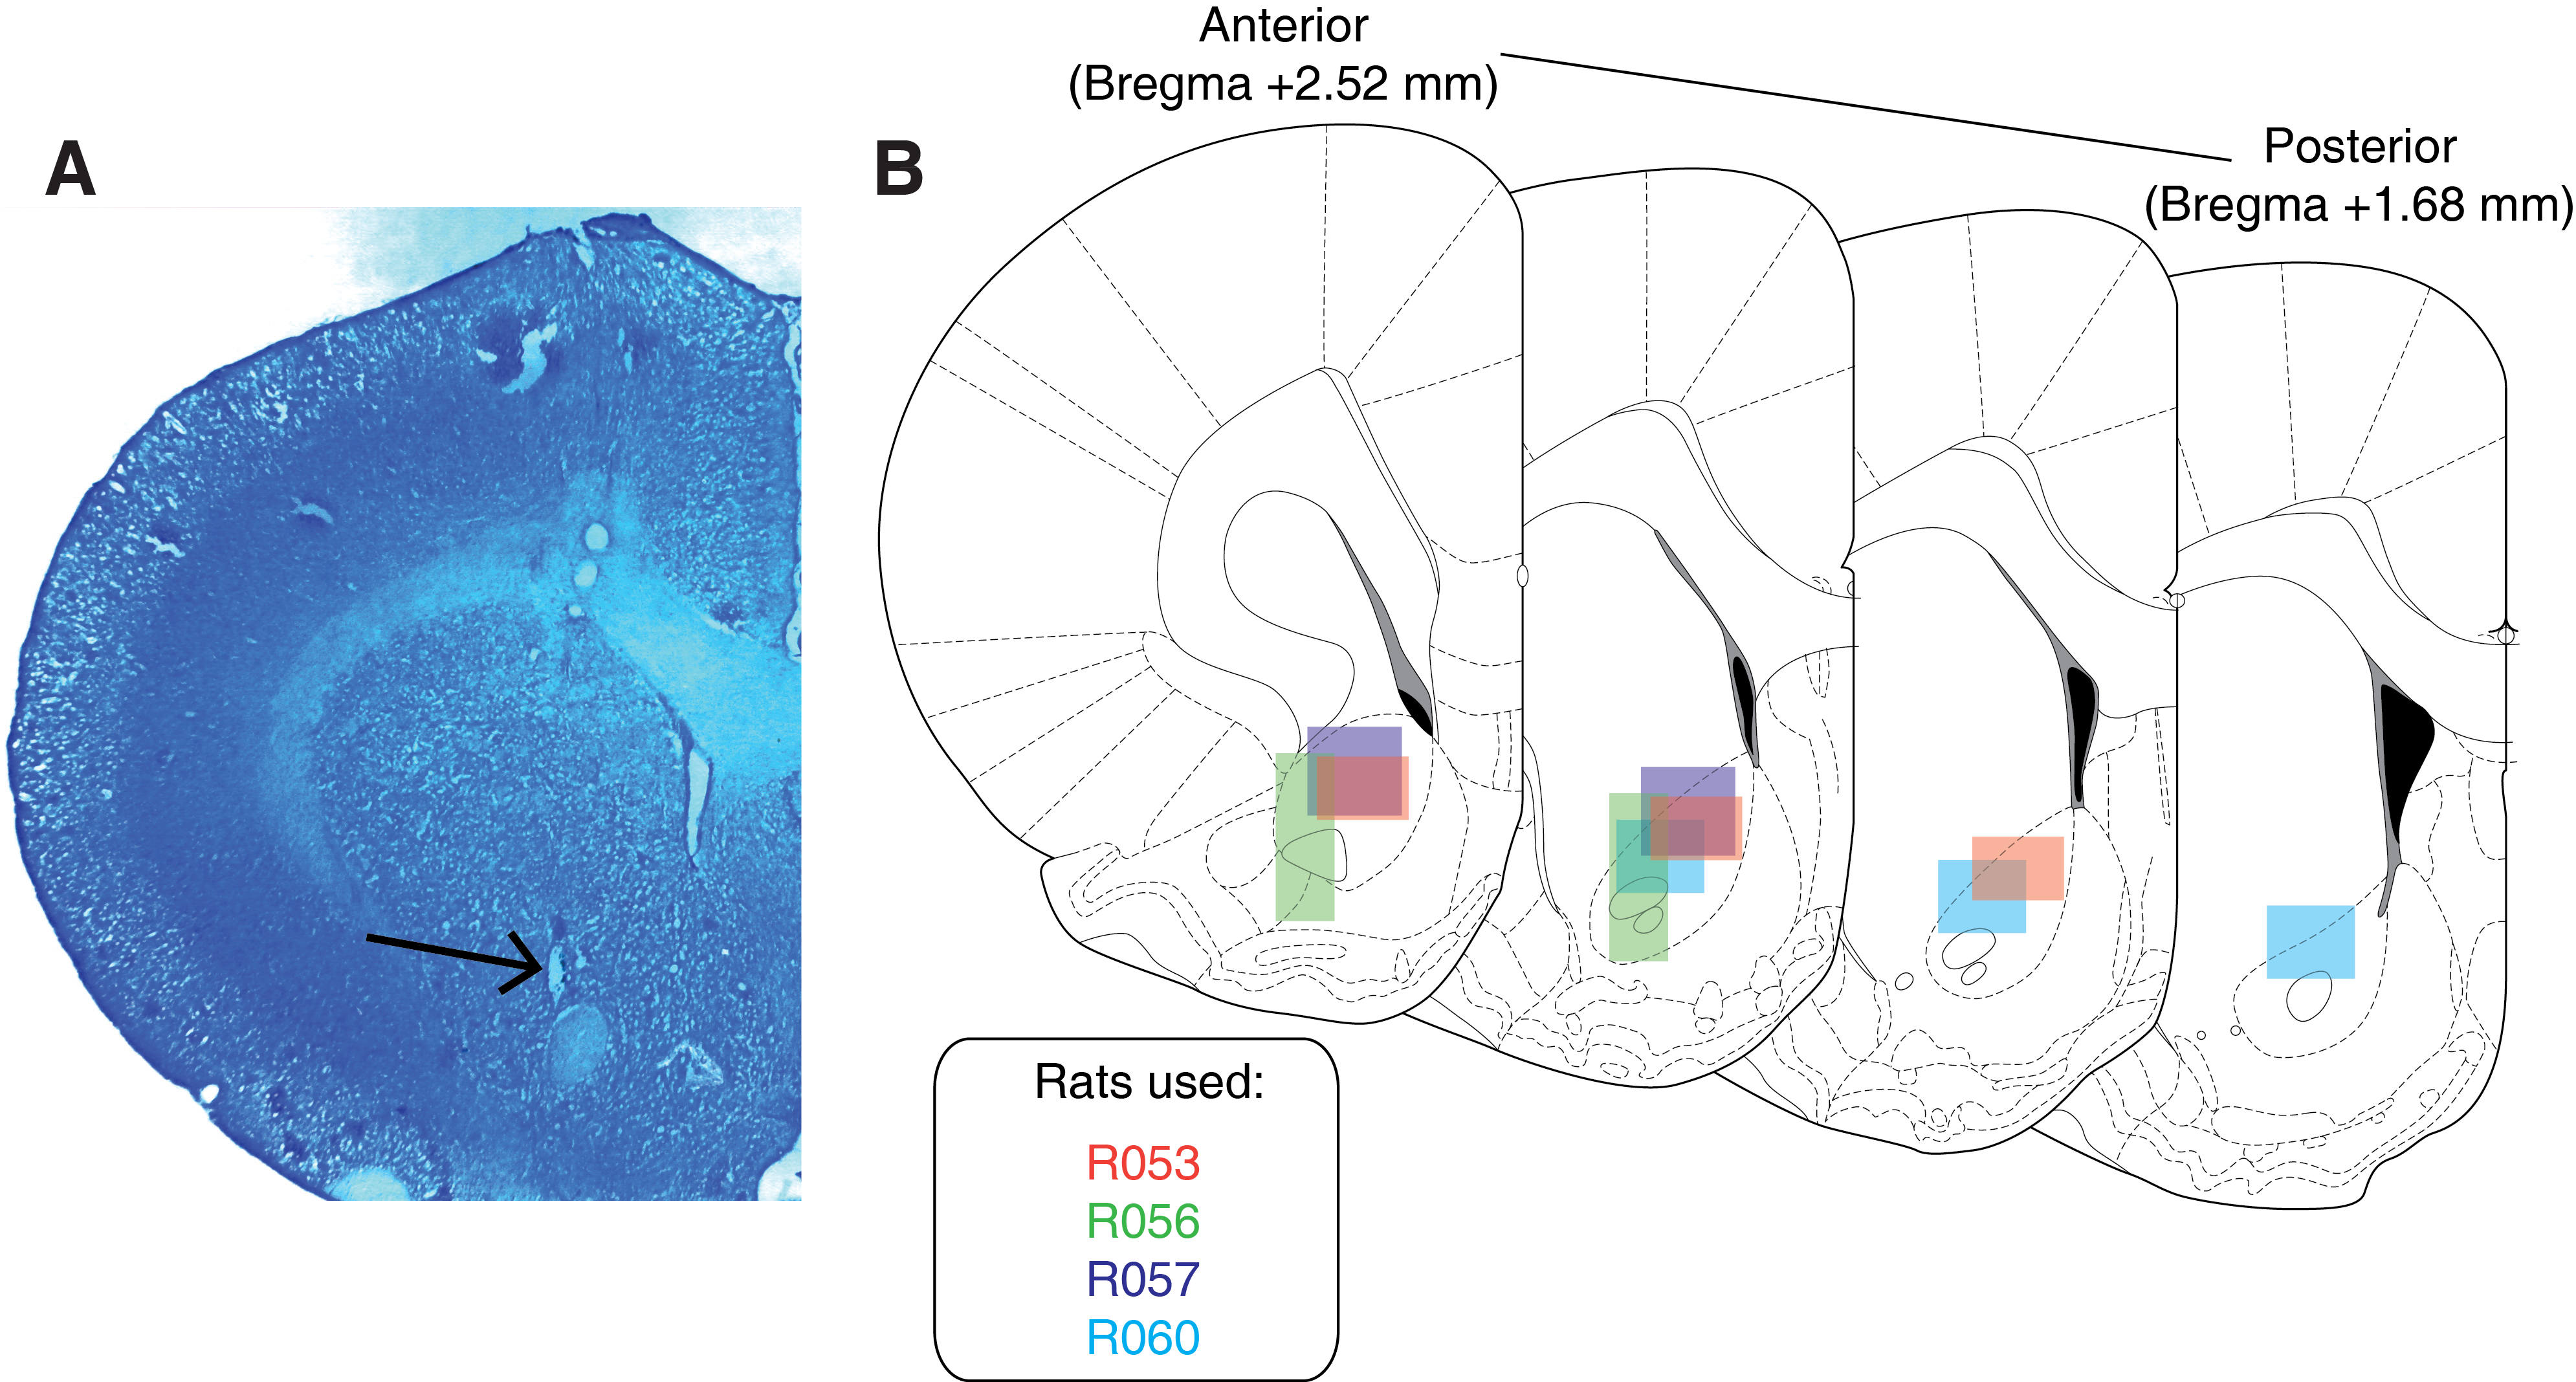
\includegraphics[width=\textwidth]{Fig 3 - Histology.png}
\caption{Histological verification of recording sites. Upon completion of
  experiments, brains were sectioned and tetrode placement was
  confirmed. \bsf{A}: Example section from R060 showing a recording site in the
  NAc core just dorsal to the anterior commissure (arrow). \bsf{B}:
  Schematic showing recording areas for all subjects.}
\label{fig:histo}
\end{figure} \clearpage

\bibliography{vStrCueCoding}
\end{document}
